\documentclass[11pt,fleqn, openany]{book} % Default font size and left-justified equations

%%%%%%%%%%%%%%%%%%%%%%%%%%%%%%%%%%%%%%%%%
% The Legrand Orange Book
% Structural Definitions File
% Version 2.1 (26/09/2018)
%
% Original author:
% Mathias Legrand (legrand.mathias@gmail.com) with modifications by:
% Vel (vel@latextemplates.com)
% 
% This file was downloaded from:
% http://www.LaTeXTemplates.com
%
% License:
% CC BY-NC-SA 3.0 (http://creativecommons.org/licenses/by-nc-sa/3.0/)
%
%%%%%%%%%%%%%%%%%%%%%%%%%%%%%%%%%%%%%%%%%

%----------------------------------------------------------------------------------------
%	VARIOUS REQUIRED PACKAGES AND CONFIGURATIONS
%----------------------------------------------------------------------------------------

\usepackage[table]{xcolor}

\usepackage{graphicx}
\usepackage{tabularx} % Required for including pictures
\usepackage{pgf,tikz,tkz-tab,eurosym,yhmath, stmaryrd}
\usepackage{pgfplots}
\usepackage{mathrsfs}
\usetikzlibrary{patterns}
\usetikzlibrary{trees}
\graphicspath{{../../Pictures/}}
\usepackage{multicol} 


\usepackage[english]{babel} % English language/hyphenation
\usepackage{icomma}
\usepackage{enumitem} % Customize lists
\setlist{nolistsep, nosep, nolistsep} % Reduce spacing between bullet points and numbered lists

\usepackage{booktabs} % Required for nicer horizontal rules in tables

 % Required for specifying colors by name


\definecolor{ocre}{RGB}{243,102,25} % Define the orange color used for highlighting throughout the book

\usepackage{listings}

\definecolor{codegreen}{rgb}{0,0.6,0}
\definecolor{codegray}{rgb}{0.5,0.5,0.5}
\definecolor{codepurple}{rgb}{0.58,0,0.82}
\definecolor{backcolour}{rgb}{0.95,0.95,0.92}

\lstdefinestyle{mystyle}{
    backgroundcolor=\color{backcolour},   
    commentstyle=\color{codegreen},
    keywordstyle=\color{magenta},
    numberstyle=\tiny\color{codegray},
    stringstyle=\color{codepurple},
    basicstyle=\ttfamily\footnotesize,
    breakatwhitespace=false,         
    breaklines=true,                 
    captionpos=b,                    
    keepspaces=true,                 
    numbers=left,                    
    numbersep=5pt,                  
    showspaces=false,                
    showstringspaces=false,
    showtabs=false,                  
    tabsize=2
}

\lstset{style=mystyle}

%----------------------------------------------------------------------------------------
% Paramétrage XSIM
%----------------------------------------------------------------------------------------

\usepackage[no-files]{xsim}


\DeclareExerciseEnvironmentTemplate{myex}{%
    \textbf{%
      \hypertarget{ex:\ExerciseID}{\sffamily{\ensuremath{\blacktriangleright}} Exercice \GetExerciseProperty{counter} \GetExerciseProperty{subtitle} --}
      \hyperlink{sol:\ExerciseID}{Voir le corrigé}%
    }\par
}{\par\smallskip}

\DeclareExerciseEnvironmentTemplate{mysol}{%
    \textbf{%
      \hypertarget{sol:\ExerciseID}{\sffamily{\ensuremath{\blacktriangleright}} Correction \GetExerciseProperty{counter} --}
      \hyperlink{ex:\ExerciseID}{Voir l'énoncé}%
    }\par
}{\par\medskip}

\xsimsetup{
  exercise/template = myex ,
  solution/template = mysol 
}

%Collection exercices

\DeclareExerciseTagging{topic}

\xsimsetup{collect}

%----------------------------------------------------------------------------------------
% SYMBOLES
%----------------------------------------------------------------------------------------

\newcommand\imCMsym[4][\mathord]{%
  \DeclareFontFamily{U} {#2}{}
  \DeclareFontShape{U}{#2}{m}{n}{
    <-6> #25
    <6-7> #26
    <7-8> #27
    <8-9> #28
    <9-10> #29
    <10-12> #210
    <12-> #212}{}
  \DeclareSymbolFont{CM#2} {U} {#2}{m}{n}
  \DeclareMathSymbol{#4}{#1}{CM#2}{#3}
}
\newcommand\alsoimCMsym[4][\mathord]{\DeclareMathSymbol{#4}{#1}{CM#2}{#3}}

\imCMsym{cmmi}{124}{\CMjmath}

\newcommand{\Oij}{(O\,;\,\vec{\imath}\,,\, \vec{\CMjmath} )}
\newcommand{\Oijk}{(O\,;\,\vec{\imath}\,,\, \vec{\CMjmath}\,,\,\vec{k})}

\newcommand\e{\mathrm{e}}
\newcommand\R{\mathbb{R}}
\newcommand\N{\mathbb{N}}


%----------------------------------------------------------------------------------------
%	MARGINS
%----------------------------------------------------------------------------------------

\usepackage{geometry} % Required for adjusting page dimensions and margins

\geometry{
	paper=a4paper, % Paper size, change to letterpaper for US letter size
	top=3cm, % Top margin
	bottom=3cm, % Bottom margin
	left=2cm, % Left margin
	right=2cm, % Right margin
	headheight=14pt, % Header height
	footskip=1.4cm, % Space from the bottom margin to the baseline of the footer
	headsep=10pt, % Space from the top margin to the baseline of the header
	%showframe, % Uncomment to show how the type block is set on the page
}

\setlength{\parindent}{0pt}
\parskip=5pt



%----------------------------------------------------------------------------------------
%	FONTS
%----------------------------------------------------------------------------------------

\usepackage{avant} % Use the Avantgarde font for headings
\usepackage{times} % Use the Times font for headings
\usepackage{mathptmx} % Use the Adobe Times Roman as the default text font together with math symbols from the Sym­bol, Chancery and Com­puter Modern fonts

%\usepackage{microtype} % Slightly tweak font spacing for aesthetics
%\usepackage[utf8]{inputenc} % Required for including letters with accents
\usepackage[T1]{fontenc} % Use 8-bit encoding that has 256 glyphs

%----------------------------------------------------------------------------------------
%	BIBLIOGRAPHY AND INDEX
%----------------------------------------------------------------------------------------

\usepackage[style=numeric,citestyle=numeric,sorting=nyt,sortcites=true,autopunct=true,babel=hyphen,hyperref=true,abbreviate=false,backref=true,backend=biber]{biblatex}
\addbibresource{bibliography.bib} % BibTeX bibliography file
\defbibheading{bibempty}{}

\usepackage{calc} % For simpler calculation - used for spacing the index letter headings correctly
\usepackage{makeidx} % Required to make an index
\makeindex % Tells LaTeX to create the files required for indexing

%----------------------------------------------------------------------------------------
%	MAIN TABLE OF CONTENTS
%----------------------------------------------------------------------------------------

\usepackage{titletoc} % Required for manipulating the table of contents

\contentsmargin{0cm} % Removes the default margin

% Part text styling (this is mostly taken care of in the PART HEADINGS section of this file)
\titlecontents{part}
	[0cm] % Left indentation
	{\addvspace{20pt}\bfseries} % Spacing and font options for parts
	{}
	{}
	{}

% Chapter text styling
\titlecontents{chapter}
	[1.25cm] % Left indentation
	{\addvspace{12pt}\large\sffamily\bfseries} % Spacing and font options for chapters
	{\color{ocre!60}\contentslabel[\Large\thecontentslabel]{1.25cm}\color{ocre}} % Formatting of numbered sections of this type
	{\color{ocre}} % Formatting of numberless sections of this type
	{\color{ocre!60}\normalsize\;\titlerule*[.5pc]{.}\;\thecontentspage} % Formatting of the filler to the right of the heading and the page number

% Section text styling
\titlecontents{section}
	[1.25cm] % Left indentation
	{\addvspace{3pt}\sffamily\bfseries} % Spacing and font options for sections
	{\contentslabel[\thecontentslabel]{1.25cm}} % Formatting of numbered sections of this type
	{} % Formatting of numberless sections of this type
	{\hfill\color{black}\thecontentspage} % Formatting of the filler to the right of the heading and the page number

% Subsection text styling
\titlecontents{subsection}
	[1.25cm] % Left indentation
	{\addvspace{1pt}\sffamily\small} % Spacing and font options for subsections
	{\contentslabel[\thecontentslabel]{1.25cm}} % Formatting of numbered sections of this type
	{} % Formatting of numberless sections of this type
	{\ \titlerule*[.5pc]{.}\;\thecontentspage} % Formatting of the filler to the right of the heading and the page number

% Figure text styling
\titlecontents{figure}
	[1.25cm] % Left indentation
	{\addvspace{1pt}\sffamily\small} % Spacing and font options for figures
	{\thecontentslabel\hspace*{1em}} % Formatting of numbered sections of this type
	{} % Formatting of numberless sections of this type
	{\ \titlerule*[.5pc]{.}\;\thecontentspage} % Formatting of the filler to the right of the heading and the page number

% Table text styling
\titlecontents{table}
	[1.25cm] % Left indentation
	{\addvspace{1pt}\sffamily\small} % Spacing and font options for tables
	{\thecontentslabel\hspace*{1em}} % Formatting of numbered sections of this type
	{} % Formatting of numberless sections of this type
	{\ \titlerule*[.5pc]{.}\;\thecontentspage} % Formatting of the filler to the right of the heading and the page number

%----------------------------------------------------------------------------------------
%	MINI TABLE OF CONTENTS IN PART HEADS
%----------------------------------------------------------------------------------------

% Chapter text styling
\titlecontents{lchapter}
	[0em] % Left indentation
	{\addvspace{15pt}\large\sffamily\bfseries} % Spacing and font options for chapters
	{\color{ocre}\contentslabel[\Large\thecontentslabel]{1.25cm}\color{ocre}} % Chapter number
	{}  
	{\color{ocre}\normalsize\sffamily\bfseries\;\titlerule*[.5pc]{.}\;\thecontentspage} % Page number

% Section text styling
\titlecontents{lsection}
	[0em] % Left indentation
	{\sffamily\small} % Spacing and font options for sections
	{\contentslabel[\thecontentslabel]{1.25cm}} % Section number
	{}
	{}

% Subsection text styling (note these aren't shown by default, display them by searchings this file for tocdepth and reading the commented text)
\titlecontents{lsubsection}
	[.5em] % Left indentation
	{\sffamily\footnotesize} % Spacing and font options for subsections
	{\contentslabel[\thecontentslabel]{1.25cm}}
	{}
	{}

%----------------------------------------------------------------------------------------
%	HEADERS AND FOOTERS
%----------------------------------------------------------------------------------------


\usepackage{fancyhdr} % Required for header and footer configuration

\pagestyle{fancy}
\renewcommand{\chaptermark}[1]{\markboth{\sffamily\normalsize\bfseries\ \thechapter.\ #1}{}} % Chapter text font settings
\renewcommand{\sectionmark}[1]{\markright{\sffamily\normalsize\thesection\hspace{5pt}#1}{}} % Section text font settings
\fancyhf{} \fancyhead[LE,RO]{\sffamily\normalsize\thepage} % Font setting for the page number in the header
\fancyhead[LO]{\rightmark} % Print the nearest section name on the left side of odd pages
\fancyhead[RE]{\leftmark} % Print the current chapter name on the right side of even pages

\fancyfoot[L]{Jason LAPEYRONNIE}
\fancyfoot[R]{\href{http://mathoutils.fr}{http://mathoutils.fr}} % Uncomment to include a footer

\renewcommand{\headrulewidth}{0.5pt} % Thickness of the rule under the header
\renewcommand{\footrulewidth}{0.5pt} % Thickness of the rule under the header

\fancypagestyle{plain}{% Style for when a plain pagestyle is specified
	\fancyhead{}\renewcommand{\headrulewidth}{0pt}%
}

% Removes the header from odd empty pages at the end of chapters
\makeatletter
\renewcommand{\cleardoublepage}{
\clearpage\ifodd\c@page\else
\hbox{}
\vspace*{\fill}
\thispagestyle{empty}
\newpage
\fi}

%----------------------------------------------------------------------------------------
%	THEOREM STYLES
%----------------------------------------------------------------------------------------

\usepackage{amsmath,amsfonts,amssymb,amsthm} % For math equations, theorems, symbols, etc

\newcommand{\intoo}[2]{\mathopen{]}#1\,;#2\mathclose{[}}
\newcommand{\ud}{\mathop{\mathrm{{}d}}\mathopen{}}
\newcommand{\intff}[2]{\mathopen{[}#1\,;#2\mathclose{]}}
\renewcommand{\qedsymbol}{$\blacksquare$}
\newtheorem{notation}{Notation}[section]

% Boxed/framed environments
\newtheoremstyle{ocrenumbox}% Theorem style name
{0pt}% Space above
{0pt}% Space below
{\normalfont}% Body font
{}% Indent amount
{\small\bf\sffamily\color{ocre}}% Theorem head font
{\;:\;}% Punctuation after theorem head
{0.25em}% Space after theorem head
{\small\sffamily\color{ocre}\thmname{#1}\nobreakspace\thmnumber{\@ifnotempty{#1}{}\@upn{#2}}% Theorem text (e.g. Theorem 2.1)
\thmnote{\nobreakspace\the\thm@notefont\sffamily\bfseries\color{black}---\nobreakspace#3}} % Optional theorem note

\newtheoremstyle{blacknumex}% Theorem style name
{5pt}% Space above
{10pt}% Space below
{\normalfont}% Body font
{} % Indent amount
{\small\bf\sffamily}% Theorem head font
{\;:\;}% Punctuation after theorem head
{0.25em}% Space after theorem head
{\small\sffamily{\tiny\ensuremath{\blacksquare}}\nobreakspace\thmname{#1}\nobreakspace\thmnumber{\@ifnotempty{#1}{}\@upn{#2}}% Theorem text (e.g. Theorem 2.1)
\thmnote{\nobreakspace\the\thm@notefont\sffamily\bfseries---\nobreakspace#3}}% Optional theorem note

\newtheoremstyle{blacknumexo}% Theorem style name
{15pt}% Space above
{10pt}% Space below
{\normalfont}% Body font
{} % Indent amount
{\small\bf\sffamily}% Theorem head font
{}% Punctuation after theorem head
{0.5em}% Space after theorem head
{\small\sffamily{\ensuremath{\blacktriangleright}}\nobreakspace\thmname{#1}\nobreakspace\thmnumber{\@ifnotempty{#1}{}\@upn{#2}}% Theorem text (e.g. Theorem 2.1)
\thmnote{\nobreakspace\the\thm@notefont\sffamily\bfseries---\nobreakspace#3} \\}% Optional theorem note



\newtheoremstyle{blacknumbox} % Theorem style name
{0pt}% Space above
{5pt}% Space below
{}% Body font
{}% Indent amount
{\large\bf\sffamily}% Theorem head font
{\;:\;}% Punctuation after theorem head
{0.25em}% Space after theorem head
{\small\sffamily\thmname{#1}\nobreakspace\thmnumber{\@ifnotempty{#1}{}\@upn{#2}}% Theorem text (e.g. Theorem 2.1)
\thmnote{\nobreakspace\the\thm@notefont\sffamily\bfseries---\nobreakspace#3}}% Optional theorem note

% Non-boxed/non-framed environments
\newtheoremstyle{ocrenum}% Theorem style name
{5pt}% Space above
{5pt}% Space below
{\normalfont}% Body font
{}% Indent amount
{\small\bf\sffamily\color{ocre}}% Theorem head font
{\;:\;}% Punctuation after theorem head
{0.25em}% Space after theorem head
{\small\sffamily\color{ocre}\thmname{#1}\nobreakspace\thmnumber{\@ifnotempty{#1}{}\@upn{#2}}% Theorem text (e.g. Theorem 2.1)
\thmnote{\nobreakspace\the\thm@notefont\sffamily\bfseries\color{black}---\nobreakspace#3}} % Optional theorem note
\makeatother

% Defines the theorem text style for each type of theorem to one of the three styles above
\newcounter{dummy} 
\newcounter{thm}
\newcounter{correction}
\newcounter{qst}
\theoremstyle{ocrenumbox}
\newtheorem{theoremeT}[dummy]{Théorème}
\newtheorem{exerciseT}{Propriété}
\newtheorem{principeT}{Principe}
\theoremstyle{blacknumex}
\newtheorem{exampleT}{Exemple}
\theoremstyle{blacknumexo}
\newtheorem{exo}[thm]{Exercice}
\newtheorem{corr}[correction]{Correction}
\newtheorem{quest}[qst]{Question}
\theoremstyle{blacknumbox}
\newtheorem{vocabulary}{Vocabulary}[section]
\newtheorem{definitionT}{Définition}
\newtheorem{corollaryT}[dummy]{Corollary}
\theoremstyle{ocrenum}
\newtheorem{proofT}[dummy]{Démonstration}


%----------------------------------------------------------------------------------------
%	DEFINITION OF COLORED BOXES
%----------------------------------------------------------------------------------------

\RequirePackage[framemethod=default]{mdframed} % Required for creating the theorem, definition, exercise and corollary boxes

% Theorem box
\newmdenv[skipabove=7pt,
skipbelow=7pt,
backgroundcolor=black!5,
linecolor=ocre,
innerleftmargin=5pt,
innerrightmargin=5pt,
innertopmargin=10pt,
leftmargin=0cm,
rightmargin=0cm,
innerbottommargin=5pt]{tBox}

%Proposition box	  
\newmdenv[skipabove=7pt,
skipbelow=7pt,
rightline=false,
leftline=true,
topline=false,
bottomline=false,
backgroundcolor=ocre!10,
linecolor=ocre,
innerleftmargin=5pt,
innerrightmargin=5pt,
innertopmargin=10pt,
innerbottommargin=3pt,
leftmargin=0cm,
rightmargin=0cm,
linewidth=4pt]{eBox}	

% Definition box
\newmdenv[skipabove=7pt,
backgroundcolor=ocre!4,
skipbelow=7pt,
rightline=false,
leftline=true,
topline=false,
bottomline=false,
linecolor=ocre,
innerleftmargin=5pt,
innerrightmargin=5pt,
innertopmargin=10pt,
leftmargin=0cm,
rightmargin=0cm,
linewidth=4pt,
innerbottommargin=5pt]{dBox}	

% Corollary box
\newmdenv[skipabove=7pt,
skipbelow=7pt,
rightline=false,
leftline=true,
topline=false,
bottomline=false,
linecolor=gray,
backgroundcolor=black!5,
innerleftmargin=5pt,
innerrightmargin=5pt,
innertopmargin=5pt,
leftmargin=0cm,
rightmargin=0cm,
linewidth=4pt,
innerbottommargin=5pt]{cBox}

\newmdenv[skipabove=7pt,
skipbelow=7pt,
backgroundcolor=black!5,
innerleftmargin=5pt,
topline=false,
bottomline=false,
rightline=false,
leftline=false,
innerrightmargin=5pt,
innertopmargin=5pt,
leftmargin=0cm,
rightmargin=0cm,
innerbottommargin=5pt]{xBox}

% Creates an environment for each type of theorem and assigns it a theorem text style from the "Theorem Styles" section above and a colored box from above
\newenvironment{theorem}{\begin{tBox}\begin{theoremeT}}{\end{theoremeT}\end{tBox}}

\newenvironment{exo2}{\noindent \begin{exo}\item\relax \noindent \begin{eBox}\item\relax}{\end{eBox}\end{exo}}


\newenvironment{proposition}{\begin{eBox}\begin{exerciseT}}{\hfill{\color{ocre}}\end{exerciseT}\end{eBox}}		

\newenvironment{principe}{\begin{eBox}\begin{principeT}}{\hfill{\color{ocre}}\end{principeT}\end{eBox}}	
		  
\newenvironment{definition}{\begin{dBox}\begin{definitionT}}{\end{definitionT}\end{dBox}}	

\newenvironment{example}{\begin{xBox}\begin{exampleT}}{\hfill{\tiny\ensuremath{\blacksquare}}\end{exampleT}\end{xBox}}

\newenvironment{demonstration}{\begin{proofT}}{\hfill{\tiny\ensuremath{\square}}\end{proofT}}		
\newenvironment{corollary}{\begin{cBox}\begin{corollaryT}}{\end{corollaryT}\end{cBox}}	

%----------------------------------------------------------------------------------------
%	REMARK ENVIRONMENT
%----------------------------------------------------------------------------------------

\newenvironment{remark}{\par\vspace{5pt}\small % Vertical white space above the remark and smaller font size
\begin{list}{}{
\leftmargin=25pt % Indentation on the left
\rightmargin=15pt}\item\ignorespaces % Indentation on the right
\makebox[-2.5pt]{
\begin{tikzpicture}[overlay]
\node[draw=ocre!60,line width=1pt,circle,fill=ocre!25,font=\sffamily\bfseries,inner sep=2pt,outer sep=0pt] at (-15pt,0pt){\textcolor{ocre}{R}};\end{tikzpicture}} % Orange R in a circle
\advance\baselineskip -1pt}{\end{list}\vskip5pt} % Tighter line spacing and white space after remark

%----------------------------------------------------------------------------------------
%	SECTION NUMBERING IN THE MARGIN
%----------------------------------------------------------------------------------------

\makeatletter
\renewcommand{\@seccntformat}[1]{\llap{\textcolor{ocre}{\csname the#1\endcsname}\hspace{1em}}}                    
\renewcommand{\section}{\@startsection{section}{1}{\z@}
{-4ex \@plus -1ex \@minus -.4ex}
{1ex \@plus.2ex }
{\normalfont\LARGE\sffamily\bfseries}}
\renewcommand{\subsection}{\@startsection {subsection}{2}{\z@}
{-3ex \@plus -0.1ex \@minus -.4ex}
{0.5ex \@plus.2ex }
{\normalfont\sffamily\bfseries}}
\renewcommand{\subsubsection}{\@startsection {subsubsection}{3}{\z@}
{-2ex \@plus -0.1ex \@minus -.2ex}
{.2ex \@plus.2ex }
{\normalfont\small\sffamily\bfseries}}                        
\renewcommand\paragraph{\@startsection{paragraph}{4}{\z@}
{-2ex \@plus-.2ex \@minus .2ex}
{.1ex}
{\normalfont\small\sffamily\bfseries}}

%----------------------------------------------------------------------------------------
%	PART HEADINGS
%----------------------------------------------------------------------------------------

% Numbered part in the table of contents
\newcommand{\@mypartnumtocformat}[2]{%
	\setlength\fboxsep{0pt}%
	\noindent\colorbox{ocre!20}{\strut\parbox[c][.7cm]{\ecart}{\color{ocre!70}\Large\sffamily\bfseries\centering#1}}\hskip\esp\colorbox{ocre!40}{\strut\parbox[c][.7cm]{\linewidth-\ecart-\esp}{\Large\sffamily\centering#2}}%
}

% Unnumbered part in the table of contents
\newcommand{\@myparttocformat}[1]{%
	\setlength\fboxsep{0pt}%
	\noindent\colorbox{ocre!40}{\strut\parbox[c][.7cm]{\linewidth}{\Large\sffamily\centering#1}}%
}

\newlength\esp
\setlength\esp{4pt}
\newlength\ecart
\setlength\ecart{1.2cm-\esp}
\newcommand{\thepartimage}{}%
\newcommand{\partimage}[1]{\renewcommand{\thepartimage}{#1}}%
\def\@part[#1]#2{%
\ifnum \c@secnumdepth >-2\relax%
\refstepcounter{part}%
\addcontentsline{toc}{part}{\texorpdfstring{\protect\@mypartnumtocformat{\thepart}{#1}}{\partname~\thepart\ ---\ #1}}
\else%
\addcontentsline{toc}{part}{\texorpdfstring{\protect\@myparttocformat{#1}}{#1}}%
\fi%
\startcontents%
\markboth{}{}%
{\thispagestyle{empty}%
\begin{tikzpicture}[remember picture,overlay]%
\node at (current page.north west){\begin{tikzpicture}[remember picture,overlay]%	
\fill[ocre!20](0cm,0cm) rectangle (\paperwidth,-\paperheight);
\node[anchor=north] at (4cm,-3.25cm){\color{ocre!40}\fontsize{220}{100}\sffamily\bfseries\thepart}; 
\node[anchor=south east] at (\paperwidth-1cm,-\paperheight+1cm){\parbox[t][][t]{8.5cm}{
\printcontents{l}{0}{\setcounter{tocdepth}{1}}% The depth to which the Part mini table of contents displays headings; 0 for chapters only, 1 for chapters and sections and 2 for chapters, sections and subsections
}};
\node[anchor=north east] at (\paperwidth-1.5cm,-3.25cm){\parbox[t][][t]{15cm}{\strut\raggedleft\color{white}\fontsize{30}{30}\sffamily\bfseries#2}};
\end{tikzpicture}};
\end{tikzpicture}}%
\@endpart}
\def\@spart#1{%
\startcontents%
\phantomsection
{\thispagestyle{empty}%
\begin{tikzpicture}[remember picture,overlay]%
\node at (current page.north west){\begin{tikzpicture}[remember picture,overlay]%	
\fill[ocre!20](0cm,0cm) rectangle (\paperwidth,-\paperheight);
\node[anchor=north east] at (\paperwidth-1.5cm,-3.25cm){\parbox[t][][t]{15cm}{\strut\raggedleft\color{white}\fontsize{30}{30}\sffamily\bfseries#1}};
\end{tikzpicture}};
\end{tikzpicture}}
\addcontentsline{toc}{part}{\texorpdfstring{%
\setlength\fboxsep{0pt}%
\noindent\protect\colorbox{ocre!40}{\strut\protect\parbox[c][.7cm]{\linewidth}{\Large\sffamily\protect\centering #1\quad\mbox{}}}}{#1}}%
\@endpart}
\def\@endpart{\vfil\newpage
\if@twoside
\if@openright
\null
\thispagestyle{empty}%
\newpage
\fi
\fi
\if@tempswa
\twocolumn
\fi}

%----------------------------------------------------------------------------------------
%	CHAPTER HEADINGS
%----------------------------------------------------------------------------------------

% A switch to conditionally include a picture, implemented by Christian Hupfer
\newif\ifusechapterimage
\usechapterimagetrue
\newcommand{\thechapterimage}{}%
\newcommand{\chapterimage}[1]{\ifusechapterimage\renewcommand{\thechapterimage}{#1}\fi}%
\newcommand{\autodot}{.}
\def\@makechapterhead#1{%
{\parindent \z@ \raggedright \normalfont
\ifnum \c@secnumdepth >\m@ne
\if@mainmatter
\begin{tikzpicture}[remember picture,overlay]
\node at (current page.north west)
{\begin{tikzpicture}[remember picture,overlay]
\node[anchor=north west,inner sep=0pt] at (0,0) {\ifusechapterimage\includegraphics[width=\paperwidth]{\thechapterimage}\fi};
\draw[anchor=west] (\Gm@lmargin,-3cm) node [line width=2pt,rounded corners=15pt,draw=ocre,fill=white,fill opacity=0.5,inner sep=15pt]{\strut\makebox[22cm]{}};
\draw[anchor=west] (\Gm@lmargin+.3cm,-3cm) node {\huge\sffamily\bfseries\color{black}\thechapter\autodot~#1\strut};
\end{tikzpicture}};
\end{tikzpicture}
\else
\begin{tikzpicture}[remember picture,overlay]
\node at (current page.north west)
{\begin{tikzpicture}[remember picture,overlay]
\node[anchor=north west,inner sep=0pt] at (0,0) {\ifusechapterimage\includegraphics[width=\paperwidth]{\thechapterimage}\fi};
\draw[anchor=west] (\Gm@lmargin,-3cm) node [line width=2pt,rounded corners=15pt,draw=ocre,fill=white,fill opacity=0.5,inner sep=15pt]{\strut\makebox[22cm]{}};
\draw[anchor=west] (\Gm@lmargin+.3cm,-3cm) node {\huge\sffamily\bfseries\color{black}#1\strut};
\end{tikzpicture}};
\end{tikzpicture}
\fi\fi\par\vspace*{50\p@}}}

%-------------------------------------------

\def\@makeschapterhead#1{%
\begin{tikzpicture}[remember picture,overlay]
\node at (current page.north west)
{\begin{tikzpicture}[remember picture,overlay]
\node[anchor=north west,inner sep=0pt] at (0,0) {\ifusechapterimage\includegraphics[width=\paperwidth]{\thechapterimage}\fi};
\draw[anchor=west] (\Gm@lmargin,-3cm) node [line width=2pt,rounded corners=15pt,draw=ocre,fill=white,fill opacity=0.5,inner sep=15pt]{\strut\makebox[22cm]{}};
\draw[anchor=west] (\Gm@lmargin+.3cm,-3cm) node {\huge\sffamily\bfseries\color{black}#1\strut};
\end{tikzpicture}};
\end{tikzpicture}
\par\vspace*{50\p@}}
\makeatother

%----------------------------------------------------------------------------------------
%	LINKS
%----------------------------------------------------------------------------------------

\usepackage{hyperref}
\hypersetup{hidelinks,backref=true,pagebackref=true,hyperindex=true,colorlinks=false,breaklinks=true,urlcolor=ocre,bookmarks=true,bookmarksopen=false}

\usepackage{bookmark}
\bookmarksetup{
open,
numbered,
addtohook={%
\ifnum\bookmarkget{level}=0 % chapter
\bookmarksetup{bold}%
\fi
\ifnum\bookmarkget{level}=-1 % part
\bookmarksetup{color=ocre,bold}%
\fi
}
}

\renewcommand*\thesection{\arabic{section}}

\newcommand*{\coord}[3]{% 
  \ensuremath{\overrightarrow{#1}\, 
    \begin{pmatrix} 
      #2\\ 
      #3 
    \end{pmatrix}}}
    
  \newcommand*{\coordb}[2]{% 
  \ensuremath{ 
    \begin{pmatrix} 
      #1\\ 
      #2 
    \end{pmatrix}}}

\newcommand*{\coorde}[4]{% 
  \renewcommand{\arraystretch}{1}\ensuremath{\overrightarrow{#1}\, 
    \begin{pmatrix} 
      #2\\ 
      #3 \\
      #4
    \end{pmatrix}}}    
  \newcommand*{\coordbe}[3]{% 
 \renewcommand{\arraystretch}{1} \ensuremath{ 
    \begin{pmatrix} 
      #1\\ 
      #2 \\
      #3
    \end{pmatrix}}}  
    
\newcommand{\Card}{\mathrm{Card}}


\DeclareExerciseCollection[topic=log01]{log01}
\DeclareExerciseCollection[topic=log02]{log02}
\DeclareExerciseCollection[topic=log03]{log03}
\DeclareExerciseCollection[topic=log04]{log04}

\begin{document}

\chapterimage{../../Pictures/background}


\chapter{Cours : Logarithme népérien}

\section{Logarithme népérien}

\begin{definition} Soit $a$ un réel strictement positif. On appelle \textit{logarithme népérien} de $a$, noté $\ln (a)$, l'unique solution de l'équation $e^x =a$, d'inconnue $x \in \mathbb{R}$.\end{definition}

\begin{demonstration}Derrière cette définition se cache une démonstration : une telle solution existe-t-elle ? Si elle existe, cette solution est-elle unique ?

La fonction $x\mapsto e^x$ est dérivable sur $\mathbb{R}$ par définition de l'exponentielle. Elle est donc continue sur $\mathbb{R}$. De plus, $\displaystyle \lim _{x \to -\infty} e^x = 0$ et $\displaystyle \lim _{x \to -\infty} e^x = +\infty$. Ainsi, d'après le théorème des valeurs intermédiaires, pour tout réel $a \in ]0;+\infty[$, il existe un réel $x$ tel que $e^x = a$.

La fonction exponentielle étant par ailleurs strictement monotone sur $\mathbb{R}$, cette solution est unique.\end{demonstration}

\begin{example}$\ln (1)=0$. En effet, l'unique solution de l'équation $e^x=1$ est $x=0$.\end{example}

\begin{example} $\ln(e)=1$, $\ln(e^2)=2$.\end{example}

\begin{proposition}Pour tout réel $a>0$, $e^{\ln (a)} = a$.

Pour tout réel $a$, $\ln(e^a)=a$.

\end{proposition}

\begin{demonstration}Soit $a$ un réel strictement positif. $\ln(a)$ est, par définition, solution de l'équation $e^x=a$. On a donc $e^{\ln(a)}=a$.

Par ailleurs, pour tout réel $a$, $e^a>0$. Par définition du logarithme népérien, $\ln(e^a)$ est l'unique solution de l'équation $e^x=e^a$, d'inconnue $x\in \mathbb{R}$. Or, $x=a$ est une solution de cette équation. On a donc $\ln (e^a)=a$.
\end{demonstration}


\begin{example}On cherche à résoudre l'équation $3e^x-6=0$, d'inconnue $x\in \mathbb{R}$. Or, pour $x\in \mathbb{R}$,
\[ 3e^x-6=0 \Leftrightarrow 3e^x=6 \Leftrightarrow e^x=2 \Leftrightarrow x = \ln (2). \]\end{example}


\textbf{Attention} : il n'existe pas de logarithme népérien de réels négatifs !

\begin{example}On cherche à résoudre l'équation $\ln(x+2)+3=0$. $\ln(x+2)$ n'existe que si $x+2>0$, c'est-à-dire $x>-2$. Soit donc $x>-2$. 
\[\ln(x+2)+3=0 \Leftrightarrow \ln(x+2)=-3 \Leftrightarrow x+2 =e^{-3} \Leftrightarrow x =e^{-3}-2.\]

Puisque $e^{-3}>0$, on a alors $e^{-3}-2>-2$. L'unique solution de l'équation est donc $e^{-3}-2$.
\end{example}
\newpage

\section{Propriétés algébriques}

\begin{proposition}Soit $a$ et $b$ des réels strictement positifs. On a
\[\ln (ab)=\ln(a)+\ln (b).\]\vspace{-0.5cm}\end{proposition}

\begin{demonstration}
Soit $a$ et $b$ des réels strictement positifs. On a
\[e^{\ln(ab)}=ab=e^{\ln(a)} \times e^{\ln (b)} = e^{\ln(a) + \ln(b)}.\] 
En appliquant $\ln$ à cette égalité, on a donc $\ln(ab)=\ln(a) + \ln(b)$.
\end{demonstration}

\begin{example}On a $\ln(2)+\ln(3)+\ln(4)=\ln(2\times 3 \times 4)=\ln(24)$.\end{example}

\begin{example}Soit $x$ un réel. Alors,
\[\ln(1+e^{-x})+x= \ln(1+e^{-x})+\ln(e^x)=\ln((1+e^{-x})e^x)=\ln(e^x+1).\]\end{example}

\begin{proposition}Soit $a$ et $b$ des réels strictement positifs. Alors,
\[\ln\left(\dfrac{1}{a}\right)=-\ln(a) \qquad \qquad \ln (ab)=\ln(a)+\ln (b).\]\vspace{-0.5cm}\end{proposition}

\begin{demonstration}Puisque $\ln(1)=0$, on a $\ln \left(a \times \dfrac{1}{a}\right)=0$, et donc, d'après la propriété précédente, $\ln(a) + \ln \left(\dfrac{1}{a}\right)=0$. Ainsi, $\ln \left(\dfrac{1}{a}\right)=-\ln(a).$

Par ailleurs, $\ln\left(\dfrac{a}{b}\right)=\ln\left(a \times \dfrac{1}{b}\right)=\ln(a)+\ln\left(\dfrac{1}{b}\right)=\ln(a)-\ln(b)$.\end{demonstration}

\begin{example}On a $\ln(21)-\ln(7)=\ln\left(\dfrac{21}{7}\right)=\ln(3)$.\end{example}

\begin{proposition}Soit $a$ un réel strictement positif. Alors,
\[\ln (\sqrt{a})=\dfrac{1}{2}\ln(a).\]\vspace{-0.5cm}\end{proposition}

\begin{demonstration}Puisque pour tout réel $a>0$, $a=\sqrt{a} \times \sqrt{a}$, on a \[\ln(a)=\ln(\sqrt{a} \times \sqrt{a})=\ln( \sqrt{a})+ \ln(\sqrt{a})=2\ln(\sqrt{a})\] et donc $\ln(\sqrt{a})=\dfrac{1}{2}\ln(a)$.\end{demonstration}

\begin{proposition}Soit $a$ un réel strictement positif. Pour tout entier \textbf{relatif} $n$
\[\ln(a^n)=n\,\ln(a).\]\vspace{-0.5cm}\end{proposition}

\begin{demonstration}Pour tout entier naturel $n$, on pose $\mathcal{P}(n)$ la proposition $\ln(a^n)=n\,\ln(a)$.
\begin{itemize}
\item \textbf{Initialisation} : $\ln(a^0)=\ln(1)=0$ et $0 \times \ln(a)=0$. $\mathcal{P}(0)$ est donc vraie.
\item \textbf{Hérédité} : Soit $n \in \mathbb{N}$. Supposons que $\mathcal{P}(n)$ est vraie. 

Alors $\ln(a^{n+1})=\ln(a^n \times a)=\ln(a^n)+\ln(a)=n\,\ln(a)+\ln(a)=(n+1)\ln(a)$. 

$\mathcal{P}(n+1)$ est vraie : $\mathcal{P}$ est héréditaire.
\item \textbf{Conclusion} : D'après le principe de récurrence, $\mathcal{P}(n)$ est vraie pour tout entier naturel $n$.
\end{itemize}
Par ailleurs, pour tout entier naturel $n$, $a^n \times a^{-n}=a^0=1$. Ainsi, $\ln(a^n \times a^{-n})=\ln(a^n)+\ln(a^{-n})=0$. On a donc $\ln(a^{-n})=-\ln(a^n)$. Or, $\ln(a^n)=n\, \ln(a)$. On a donc $\ln(a^{-n})=-n\, \ln(a)$.
\end{demonstration}

\begin{example}On souhaite simplifier $\ln(12)+\ln(3)-2\ln(6)$.

$\begin{array}{rcl}\ln(12)+\ln(3)-2\ln(6)&=&\ln(12 \times 3)-2\ln(6)\\&=&\ln(36)-2\ln(6)\\&=&\ln(6^2)-2\ln(6)\\&=&2\ln(6)-2\ln(6)=0.\end{array}$\end{example}

\begin{example}On a $\dfrac{\ln(10000)}{\ln(0.001)}=\dfrac{\ln(10^4)}{\ln(10^{-3}}=\dfrac{4ln(10)}{-3\ln(10)}=-\dfrac{4}{3}$.\end{example}


\section{Fonction logarithme népérien}


\begin{definition}On appelle \textit{fonction logarithme népérien} la fonction $x\mapsto \ln(x)$ définie pour tout réel $x$ strictement positif.

Cette fonction est la \textit{fonction réciproque} de la fonction exponentielle.\end{definition}

\subsection{Limites}

\begin{proposition}On a les limites suivantes :
\[ \lim_{x\to 0^+}\ln(x)=-\infty \quad\text{et} \lim_{x\to +\infty} \ln(x) = +\infty \]
De plus, pour tout entier naturel $n$,
\[ \lim_{x\to 0^+}x^n\,\ln(x) = 0\quad \text{et}\lim_{x\to +\infty} \dfrac{\ln(x)}{x^n}=0\]
La puissance de $x$ l'emporte sur le logarithme en cas d'indéterminée : ce sont les croissances comparées au logarithme.\end{proposition}

\begin{demonstration}[Au programme : $ \displaystyle\lim_{x\to 0^+}x\,\ln(x)$]

Pour $x>0$, posons $X=\ln(x)$. 

Ainsi, $x\,\ln(x)=e^X \times X$. Or, $\displaystyle\lim_{x\to 0^+}\ln(x)=-\infty$ et, par croissances comparées, $\displaystyle\lim_{X\to -\infty}Xe^X=0$. Par composition de limite, $ \displaystyle\lim_{x\to 0^+}x\,\ln(x)=0$. \end{demonstration}

\newpage

\subsection{Dérivabilité}


\begin{proposition}La fonction $\ln$ est dérivable sur $]0;+\infty[$ et pour tout réel $x>0$, $\ln'(x)=\dfrac{1}{x}$.\end{proposition}

La fonction $\ln$ est donc également continue sur $]0;+\infty[$.

\begin{demonstration}[Au programme]On admet que $\ln$ est dérivable sur $]0;+\infty[$.

Pour tout réel $x>0$, on pose $f(x)=e^{\ln(x)}$. $f$ est dérivable sur $]0;+\infty[$.
\begin{itemize}
\item D'une part, on sait que pour tout réel $x>0$, $f'(x)=1$.
\item D'autre part, en utilisant la formule de la dérivée d'une fonction composée, on sait que 
\[f'(x)=\ln'(x) \times e^{\ln(x)}=\ln'(x) \times x.\]
\end{itemize}
Ainsi, pour tout $x>0$, $\ln'(x) \times x=1$ et donc $\ln'(x)=\dfrac{1}{x}$.\end{demonstration}

\begin{example}Pour tour réel $x>0$, on pose $f(x)=e^x \ln(x)$.

\begin{itemize}
\item Pour tout réel $x$, on pose $u(x)=e^{x}$. $u$ est dérivable sur $]0;+\infty[$ et pour tout réel $x>0$, $u'(x)=e^x$.
\item Pour tout réel $x$, on pose $v(x)=\ln (x)$. $v$ est dérivable sur $]0;+\infty[$ et pour tout réel $x>0$, $v'(x)=\dfrac{1}{x}$.
\end{itemize}
Ainsi, $f$ est dérivable sur $]0;+\infty[$ comme produit de fonctions dérivables sur cet intervalle. De plus, pour tout réel $x>0$
\[ f'(x)=u'(x) \times v(x) + u(x) \times v'(x)=e^x \times \ln(x) + e^x \times \dfrac{1}{x}= \dfrac{e^x(x\ln(x)+1)}{x}.\]\end{example}

On en déduit naturellement la propriété suivante.

\begin{proposition}Soit $u$ une fonction définie sur un intervalle $I$ telle que pour tout réel $x\in I$, $u(x)>0$. 

Alors $\ln(u)$ est dérivable et $(\ln(u))'=\dfrac{u'}{u}$\end{proposition}

\begin{example}Pour tout réel $x$, on pose $u(x)=x^2-2x+5$ et  $f(x)=\ln(u(x))=\ln(x^2-2x+5)$.

Il faut avant tout vérifier que pour tout réel $x$, $u(x)>0$ ! Sans quoi, la fonction $f$ ne serait pas définie sur $\mathbb{R}$.

Or, $u$ une fonction polynôme du second degré dont le discriminant $\Delta$ vaut $(-2)^2-4\times 1 \times 5 = -16>0$. Ainsi, pour tout réel $x$, $u(x)$ est du signe du coefficient dominant, 1, c'est-à-dire $u(x)>0$.

Par ailleurs, la fonction $u$ est dérivable sur $\mathbb{R}$ et pour tout réel $x$, $u'(x)=2x-2$.

Ainsi, $f$ est dérivable sur $\mathbb{R}$ et pour tout réel $x$, 
\[ f'(x)=\dfrac{u'(x)}{u(x)}=\dfrac{2x-2}{x^2-2x+5}.\]
\end{example}

Puisque $\ln(u)$ n'est définie que lorsque $u$ est strictement positive, on en déduit que $u$ et $\ln(u)$ ont les mêmes variations.
\newpage
\subsection{Étude de la fonction $\ln$}

\begin{proposition}La fonction $\ln$ est strictement croissante sur $]0;+\infty [$.\end{proposition}

\begin{demonstration}La fonction $\ln$ est dérivable sur $]0;+\infty[$ et pour tout réel $x>0$, $\ln'(x)=\dfrac{1}{x}$ qui est strictement positif. $\ln$ est donc strictement croissante.\end{demonstration}

La stricte croissance du logarithme nous est notamment utile pour déterminer le signe d'une expression mettant en jeu des logarithmes, et en particulier...

\begin{proposition}Soit $x$ et $y$ deux réels strictement positifs. Alors $\ln(x)\geqslant\ln(y)$ si et seulement si $x\geqslant y$.
En particulier, $\ln(x) \geqslant 0$ si et seulement si $x\geqslant 1$.\end{proposition}

\begin{example}On souhaite déterminer l'entier $n$ à partir duquel $3-12 \times 0.9^n \geqslant 2.9$.

En soustrayant trois aux deux membres de cette inégalité, on obtient $-12 \times 0.9^n \geqslant -0.1$. En divisant alors par $-12$ qui est négatif, on a alors $0.9^n \leqslant \dfrac{1}{120}$.

L'inconnu que nous cherchons est en exposant et les deux quantités dans cette inégalité sont strictement positives, nous allons donc pouvoir utiliser le logarithme népérien. 

Puisque la fonction logarithme népérien est strictement croissante sur $]0;+\infty[$,  $0.9^n \leqslant \dfrac{1}{120}$ si et seulement si $\ln(0.9^n) \leqslant \ln\left(\dfrac{1}{120}\right)$, soit $n\ln(0.9) \leqslant -\ln(120)$. 

Puisque $0.9<1$, on a $\ln(0.9) < 0$. En divisant l'inégalité par $\ln(0.9)$, \textbf{il faudra donc changer son sens !}

Ainsi, $n\ln(0.9) \leqslant -\ln(120)$ si et seulement si $n \geqslant -\dfrac{\ln(120)}{\ln(0.9)}$.

Or, $-\dfrac{\ln(120)}{\ln(0.9)} \simeq 45.4$. Le premier entier $n$ tel que $3-12 \times 0.9^n \geqslant 2.9$ est donc $n=46$.\end{example}

\begin{proposition}La courbe de la fonction $\ln$ est symétrique à la courbe de la fonction $\exp$ par rapport à la droite d'équation $y=x$.\end{proposition}

\begin{center}
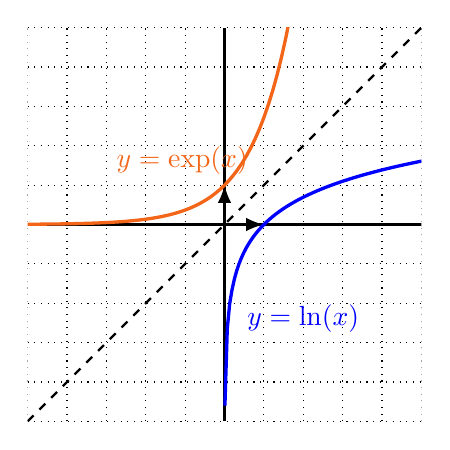
\begin{tikzpicture}[scale=0.5]
\clip (-5,-5) rectangle (5,5);
\draw [thin, dotted] (-5,-5) grid (5,5);
\draw [thick] (-5,0)--(7,0);
\draw [thick] (0,-5) -- (0,5);
\draw [very thick,->,>=latex] (0,0)--(0,1);
\draw [very thick,->,>=latex] (0,0)--(1,0);
\draw [very thick, ocre,domain=-5:6,samples=100] plot (\x,{exp(\x)});
\draw [very thick, blue,domain=0.01:6,samples=100] plot (\x,{ln(\x)});
\draw [ thick, dashed,domain=-5:6,samples=100] plot (\x,{\x});
\draw [thick,ocre] (-3,1) node[above right] {$y=\exp(x)$};
\draw [thick, blue] (2,-3) node[above] {$y=\ln(x)$};
\end{tikzpicture}
\end{center}

Cette propriété est vraie pour toutes les fonctions réciproques l'une de l'autre. Par exemple, vous pouvez observer le même phénomène en regardant les courbes des fonctions $x\mapsto x^2$ et $x\mapsto \sqrt{x}$ sur $[0;+\infty[$. Autre exemple, la fonction inverse, qui est sa propre réciproque. La courbe de cette fonction est elle-même symétrique par rapport à la droite d'équation $y=x$.

\chapter{Exercices}

\section*{Logarithme népérien}

\begin{exercise}[topic=log01]Résoudre les équations suivantes en précisant leur domaine de résolution.

\renewcommand{\arraystretch}{1.5}
 \begin{tabularx}{\linewidth}{XXX}
 \textbf{a.} $2\ln(x)+1=3$ & \textbf{b.} $\ln(3x-4)=0$ &\textbf{c.} $e^{3x+2}=4$\\
\textbf{d.}  $2+3\ln(3x-2)=-1$ &\textbf{e.}  $\ln(e^{3x+4})=5$ &\textbf{g.}  $e^{2x-3}=3-\pi$ \\
 \textbf{h.} $(e^{2x}-3)(e^x+5)=0$& \textbf{i.} $(\ln(x))^2-\ln(x)=0$ & \textbf{j.} $(e^x-1)\ln(x-e)=0$\end{tabularx}

\end{exercise}

\begin{solution}
\textbf{a.} Soit $x>0$, $2\ln(x)+1=3 \Leftrightarrow 2\ln(x)=2 \Leftrightarrow \ln(x)=1 \Leftarrow x =e$. $S=\{e\}$.

\textbf{b.} Soit $x> \dfrac{4}{3}$, $\ln(3x-4)=0 \Leftrightarrow 3x-4=1 \Leftrightarrow x=\dfrac{5}{3}$. $S=\left\{\dfrac{5}{3}\right\}$.

\textbf{c.} Soit $x\in\mathbb{R}$. $e^{3x+2}=4 \Leftrightarrow 3x+2=\ln(4) \Leftrightarrow x=\dfrac{\ln(4)-2}{3}$. $S=\left\{\dfrac{\ln(4)-2}{3}\right\}$.

\textbf{d.} Soit $x > \dfrac{2}{3}$. $2+3\ln(3x-2)=-1 \Leftrightarrow \ln(3x-2)=-1 \Leftrightarrow 3x-2 =e^{-1} \Leftrightarrow x =\dfrac{e^{-1}+2}{3}$. $S=\left\{\dfrac{e^{-1}+2}{3}\right\}$.

\textbf{e.} Soit $x\in \mathbb{R}$. $\ln(e^{3x+4})=5 \Leftrightarrow 3x+4=5 \Leftrightarrow x= \dfrac{1}{3}$. $S=\left\{\dfrac{1}{3}\right\}$.

\textbf{f.} Puisque $3-\pi <0$, l'équation $e^{2x-3}=3-\pi$ ne possède pas de solution réelle.

\textbf{g.} Soit $x\in \mathbb{R}$. $(e^{2x+1}-3)(e^x+5)=0 \Leftrightarrow e^{2x+1}-3=0  \text{ ou } e^x+5=0$.
\begin{itemize}
\item $e^{2x+1}-3=0 \Leftrightarrow e^{2x+1}=3 \Leftrightarrow 2x+1=\ln(3) \Leftrightarrow x=\dfrac{\ln(3)-1}{2}$.
\item $e^x+5=0$ est impossible puisque $e^x>0$.
\end{itemize}
Ainsi, $S=\left\{ \dfrac{\ln(3)-1}{2}\right\}$.

\textbf{h.} Soit $x>0$. $(\ln(x))^2-\ln(x)=0 \Leftrightarrow \ln(x) (\ln(x)-1)=0 \Leftrightarrow \ln(x)=0 \text{ ou } \ln(x)=1 \Leftrightarrow x=1 \text{ ou } x=e$. $S=\{1,e\}$.

\textbf{i.} Soit \(x>e\),\((x-1)\ln(x-e)=0 \Leftrightarrow x-1=0\) ou \(\ln(x-e)=0\). Or,
\begin{itemize}
\item \(x-1 = 0\Leftrightarrow x=1\). 1 n'est cependant pas une solution car il n'est pas dans l'ensemble de résolution.
\item \(\ln(x-e)=0 \Leftrightarrow x-e=1 \Leftrightarrow x=1+e\).\end{itemize}
L'unique solution de cette équation est donc \(1+e\).
\end{solution}



\begin{exercise}[topic=log01]En utilisant un changement de variable, résoudre l'équation $3e^{2x}+9e^x-30=0$ sur $\mathbb{R}$.\end{exercise}

\begin{solution}Pour tout réel $x$, on pose $X=e^x$. Ainsi, 
\[3e^{2x}+9e^x-30=0 \Leftrightarrow 3X^2+9X-30=0.\]
Cette deuxième équation est une équation du second degré. Le discriminant du polynôme $3X^2+9X-30$ vaut $441$ qui est strictement positif. Ce polynôme a donc deux racines qui sont $2$ et $-5$.

On a donc $X=2$ ou $X=-5$, c'est-à-dire $e^x = 2$ (et donc $x=\ln(2)$) ou $e^x=-5$ ce qui est impossible.

L'unique solution de l'équation est donc $\ln(2)$.\end{solution}




\begin{exercise}[topic=log01]Résoudre les inéquations suivantes. On précisera bien les domaines de résolution.

\begin{tabularx}{\linewidth}{XXX}\textbf{a.} $\ln(5x-3) \geqslant 0$ & \textbf{b.} $\ln(9x-2) < 0$ &\textbf{c.}  $\ln(3x+1) \geqslant \ln(3-x)$\end{tabularx}\end{exercise}

\begin{solution}\textbf{a.} $\ln(5x-3)$ existe si et seulement si $5x-3>0$, c'est-à-dire $x >\dfrac{5}{3}$. Soit donc \(x > \dfrac{5}{3}\). Alors, par croissance de la fonction exponentielle sur $\mathbb{R}$, \(\ln(5x-3) \geqslant 0\) si et seulement si \(5x-3 \geqslant 1\) soit \(x\geqslant \dfrac{4}{5}\). \(S = \left[\dfrac{4}{5} +\infty\right[\).

\textbf{b.} $\ln(9x-2)$ existe si et seulement si $9x-2>0$, c'est-à-dire $x >\dfrac{2}{9}$. Soit donc \(x > \dfrac{2}{9}\). Alors  par croissance de la fonction exponentielle sur $\mathbb{R}$, \(\ln(9x-2) < 0\) si et seulement si \(9x-2 < 1\) soit \(x< \dfrac{1}{3}\). Ainsi, \(S=\left]\dfrac{2}{9};\dfrac{1}{3}\right[\).

\textbf{c.} $\ln(3x+1)$ existe si et seulement si $3x+1>0$, c'est-à-dire $x >-\dfrac{1}{3}$. Par ailleurs, $\ln(3-x)$ existe si et seulement si $3-x>0$, c'est-à-dire $x<3$. Les deux expressions existent toutes deux lorsque $-\dfrac{1}{3}<x<3$. \\ Soit donc \(x \in \left]-\dfrac{1}{3};3\right[\). Alors,  par croissance de la fonction exponentielle sur $\mathbb{R}$, \(\ln(3x+1) \geqslant \ln(3-x)\) si et seulement si \(3x+1 \geqslant 3-x\) soit \(x \geqslant \dfrac{1}{2}\). Finalement, \(S=\left[\dfrac{1}{2};+\infty \right[ \cap  \left]-\dfrac{1}{3};3\right[$ soit \(S=\left[\dfrac{1}{2};3\right[\).\end{solution}




\begin{exercise}[topic=log01]
Pour tout réel $x$, on pose $sh(x)=\dfrac{e^x-e^{-x}}{2}$. Cette quantité est appelée sinus hyperbolique de $x$.

\begin{enumerate}
\item Justifier que $sh$ est deux fois dérivable sur $\mathbb{R}$ et que pour tout réel $x$, $sh''(x)=sh(x)$.

\item Pour tout réel $x$, on pose $f(x)=\ln(x+\sqrt{x^2+1})$.  Montrer que pour tout réel $x$, $(sh\circ f) (x)=x$ et $(f \circ sh) (x) = x$.

\end{enumerate}\end{exercise}

\begin{solution}$sh$ est deux fois dérivable sur $\mathbb{R}$ comme somme de fonctions dérivables sur $\mathbb{R}$. De plus, pour tout réel $x$,
\[sh'(x)=\dfrac{e^x-(-e^{-x})}{2}=\dfrac{e^x+e^{-x}}{2}\]
et
\[sh''(x)=\dfrac{e^x-e^{-x}}{2}=sh(x).\]

Pour tout  réel $x$, 
\[sh\circ f (x)=\dfrac{e^{\ln(x+\sqrt{x^2+1})}-e^{-\ln(x+\sqrt{x^2+1})}}{2}=\dfrac{x+\sqrt{x^2+1}-\dfrac{1}{x+\sqrt{x^2+1}}}{2}.\]
Ainsi
\[ sh\circ f (x)= \dfrac{(x+\sqrt{x^2+1})^2-1}{2(x+\sqrt{x^2+1})}=\dfrac{x^2+2x\sqrt{x^2+1}+x^2+1-1}{2(x+\sqrt{x^2-1}}=\dfrac{2x(x+\sqrt{x^2+1})}{2(x+\sqrt{x^2+1})}=x.\]
Par ailleurs, pour tout réel $x$,
\[ f \circ sh(x)= \ln\left( \dfrac{e^x-e^{-x}}{2}+\sqrt{\left(\dfrac{e^x-e^{-x}}{2}\right)^2+1}\right)=\ln\left( \dfrac{e^x-e^{-x}}{2}+\sqrt{\dfrac{e^{2x}-2+e^{-2x}}{4}+1}\right).\]

Or, 

\[\dfrac{e^{2x}-2+e^{-2x}}{4}+1=\dfrac{e^{2x}+2+e^{-2x}}{4}=\left(\dfrac{e^x+e^{-x}}{2}\right)^2.\]
Ainsi, 
\[f \circ sh(x) = \ln\left( \dfrac{e^x-e^{-x}}{2}+\sqrt{\left(\dfrac{e^x+e^{-x}}{2}\right)^2}\right).\]

Or, pour tout réel $x$, $e^x+e^{-x}\geqslant 0$ et donc $\sqrt{\left(\dfrac{e^x+e^{-x}}{2}\right)^2}=\dfrac{e^x+e^{-x}}{2}$. Ainsi, 

\[f \circ sh(x)=\ln\left( \dfrac{e^x-e^{-x}}{2}+\dfrac{e^x+e^{-x}}{2}\right)\ln\left(\dfrac{2e^x}{2}\right)=x.\]\end{solution}





\begin{exercise}[topic=log01]Soit $f$ la fonction $x\mapsto \dfrac{e^x-1}{e^x+1}$, définie sur $\mathbb{R}$.
\begin{enumerate}
\item Montrer que pour tout réel $y \in ]-1;1[$, il existe un unique réel $x$ tel que $y=f(x)$.
\item Soit $y\in ]-1;1[$ et $x\in\mathbb{R}$ tel que $y=f(x)$. Exprimer $x$ en fonction de $y$.
\end{enumerate}\end{exercise}

\begin{solution}D'une part, puisque $\displaystyle\lim_{x \to - \infty}e^x=0$, on a $\displaystyle\lim_{x\to-\infty}f(x)=-1$. 

Par ailleurs, pour tout réel $x$, $f(x)=\dfrac{e^x}{e^x}\times \dfrac{1-\frac{1}{e^x}}{1+\frac{1}{e^x}}=\dfrac{1-e^{-x}}{1+e^{-x}}$. Ainsi, $\displaystyle\lim_{x\to \infty}f(x)=1$.

Enfin, $f$ est continue sur $]-\infty;+\infty[$. D'après le théorème des valeurs intermédiaires, pour tout réel $y\in]-1;1[$, il existe un réel $x$ tel que $y=f(x)$.

De plus, $f$ est dérivable et pour tout réel $x$, $f'(x)=\dfrac{e^x(e^x+1)-(e^x-1)e^x}{(1+e^x)^2}=\dfrac{2e^x}{(1+e^x)^2}>0$. $f$ est donc strictement croissante sur $\mathbb{R}$. Ainsi, pour tout réel $y\in ]-1;1[$, le réel $x$ tel que $f(x)=y$ est unique.

Soit donc $y\in]-1;1[$ et $x$ le réel tel que $y=f(x)$. On a alors $y=\dfrac{e^x-1}{e^x+1}$ et donc $y(e^x+1)=e^x-1$. 

Ainsi, $ye^x+y=e^x-1$. On a alors $ye^x-e^x=-1-y$ soit $e^x(y-1)=-1-y$ et donc $e^x=\dfrac{-1-y}{y-1}=\dfrac{1+y}{1-y}$. 

Puisque $y\in]-1;1[$, on a bien $\dfrac{1+y}{1-y}>0$ puisque c'est le quotient de deux réels strictement positifs. 

Finalement, on a $x=\ln\left(\dfrac{1+y}{1-y}\right)$.\end{solution}


\printcollection{log01}

\section*{Propriétés algébriques}

\begin{exercise}[topic=log02]Simplifier les écritures suivantes.

\begin{tabularx}{0.9\linewidth}{XX}
$\ln(3)+\ln(4)-\ln(6)$ & $\dfrac{\ln(9)}{\ln(3)}-\ln(1)$ \\
$4\ln(3)-\ln(9)+2\ln(27)$ & $\ln(3x^2)-\ln(3)$ avec $x>0$
\end{tabularx}
\end{exercise}

\begin{solution}\hspace{0pt}
\begin{itemize}
\item $\ln(3)+\ln(4)-\ln(6) = \ln\left( \dfrac{3 \times 4}{6}\right)=\ln(2)$
\item $\dfrac{\ln(9)}{\ln(3)}-\ln(1)=\dfrac{\ln(3^2)}{\ln(3)}-0=\dfrac{2\ln(3)}{\ln(3)}=2$
\vskip5pt
\item $4\ln(3)-\ln(9)+2\ln(27)=4\ln(3)-\ln(3^2)+2\ln(3^3)=4\ln(3)-2\ln(3)+6\ln(3)=8\ln(3)$.
\vskip5pt
\item $\ln(3x^2)-\ln(3)=\ln(3)+\ln(x^2)-\ln(3)=\ln(x^2)=2\ln(x)$ car $x>0$
\end{itemize}\end{solution}




\begin{exercise}[topic=log02]Résoudre l'équation $\ln(4x^2)+6\ln(x)-3=0$, d'inconnue $x>0$.\newpage \end{exercise}

\begin{solution}

Pour tout $x>0$
\[ \ln(4x^2)+6\ln(x)-3=\ln(4)+\ln(x^2)+6\ln(x)-3=8\ln(x)+\ln(4)-3.\]

Ainsi
\[ \ln(4x^2)+6\ln(x)-3=0\Leftrightarrow 8\ln(x)+\ln(4)-3=0 \Leftrightarrow \ln(x)= \dfrac{3-\ln(4)}{8}\Leftrightarrow x=\exp \left( \dfrac{3-\ln(4)}{8}\right).\]
\end{solution}



\begin{exercise}[topic=log02]Montrer que pour tout réel $x>1$, $\ln(x^2-1)-\ln(x^2+2x+1)=\ln\left(\dfrac{x-1}{x+1}\right)$.\end{exercise}

\begin{solution}Pour tout réel $x>1$, 
\[ \ln(x^2-1)-\ln(x^2+2x+1) =\ln\left(\dfrac{x^2-1}{x^2+2x+1}\right)=\ln\left(\dfrac{(x-1)(x+1)}{(x+1)^2}\right)=\ln\left(\dfrac{x-1}{x+1}\right).\]\end{solution}




\begin{exercise}[topic=log02]Que vaut $\ln\left(\dfrac{1}{2}\right)+\ln\left(\dfrac{2}{3}\right)+\ln\left(\dfrac{3}{4}\right)+\ldots+\ln\left(\dfrac{49}{50}\right)$ ?\end{exercise}

\begin{solution} $\ln\left(\dfrac{1}{2}\right)+\ln\left(\dfrac{2}{3}\right)+\ln\left(\dfrac{3}{4}\right)+\ldots+\ln\left(\dfrac{49}{50}\right) = \ln \left( \dfrac{1}{2} \times \dfrac{2}{3} \times \dfrac{3}{4} \times \ldots \times \dfrac{49}{50}\right)$.

Après simplification, il reste donc 
\[ \ln\left(\dfrac{1}{2}\right)+\ln\left(\dfrac{2}{3}\right)+\ln\left(\dfrac{3}{4}\right)+\ldots+\ln\left(\dfrac{49}{50}\right)= \ln\left( \dfrac{1}{50}\right).\]\end{solution}




\begin{exercise}[topic=log02]Montrer que pour tout réel $x$, $\ln(1+e^{-x})=\ln(1+e^x)-x$.\end{exercise}

\begin{solution}Pour tout réel $x$, en factorisant dans le $\ln$ par $e^{-x}$, on a
\[\ln(1+e^{-x}) = \ln\left(e^{-x} \times \left( \dfrac{1}{e^{-x}}+1\right)\right)=\ln(e^{-x})+\ln \left( \dfrac{1}{e^{-x}}+1\right)=-x+\ln(1+e^x).\]\end{solution}




\begin{exercise}[topic=log02]On considère la suite $(u_n)$ définie par $u_0=e^3$ et pour tout entier naturel $n$, $u_{n+1}=e\sqrt{u_n}$.
\begin{enumerate}
\item Montrer que $(u_n)$ est décroissante et que pour tout entier naturel $n$, $e^2 \leqslant u_n$.
\item En déduire que $(u_n)$ converge. Quelle est sa limite ?
\item Pour tout entier naturel $n$, on pose $a_n=\ln(u_n)-2$.
\begin{enumerate}
\item Exprimer $u_n$ en fonction de $a_n$ pour tout entier naturel $n$.
\item Montrer que la suite $(a_n)$ est géométrique. On précisera sa raison et son premier terme.
\item En déduire que pour tout entier naturel $n$, $u_n=\exp \left(2 + \left(\dfrac{1}{2}\right)^n\right)$.
\item Retrouver la limite de la suite $(u_n)$ à l'aide de cette expression.
\end{enumerate}
\end{enumerate} \end{exercise}

\begin{solution}\hspace{0pt}


\begin{enumerate}
\item Pour tout entier naturel \(n\), on considère la proposition \(P(n)\) : « \(e^2 \leqslant u_{n+1} \leqslant u_n\) ».
	\begin{itemize}
	\item Initialisation : On a \(u_0=e^3\) et \(u_1=e \times \sqrt{e^3}=e^{5/2}\). On a bien \(e^2 \leqslant u_1 \leqslant e\).
		\item Soit \(n\in\mathbb{N}\) tel que \(P(n)\) est vraie. On a alors \(e^2 \leqslant u_{n+1} \leqslant u_n\). En appliquant la fonction racine carrée, qui est strictement croissante sur \([0;+\infty [\), on a alors \(e \leqslant \sqrt{u_{n+1}} \leqslant \sqrt{u_n}\). On multiplie alors par \(e\) et on obtient \(e \times e\leqslant e\sqrt{u_{n+1}} \leqslant e\sqrt{u_n}\) soit \(e^2 \leqslant u_{n+2} \leqslant u_{n+1}\). \(P(n+1)\) est donc vraie.
		\item Par récurrence, \(P(n)\) est vraie pour tout entier naturel \(n\).
		\end{itemize}
		\item Puisque la suite \((u_n)\) est décroissante et minorée, alors elle converge vers une limite que l'on note \(l\). Par ailleurs, la fonction \(x\mapsto e\sqrt{x}\) est continue sur \([e^2;+\infty[\). On a donc \(l=e\sqrt{l}\) et donc \(l=0\) ou \(l=e^2\). L'unique possibilité est alors \(l=e^2\).
		\item \begin{enumerate}\item Pour tout entier naturel \(n\), \(a_n=\ln (u_n)-2\) d'où \(\ln(u_n)=a_n+2\) et \(u_n=e^{a_n+2}\)
			\item Pour tout entier naturel \(n\),
\[a_{n+1}=\ln(u_{n+1})-2=\ln(e\sqrt{u_n})-2=\ln(e)+\ln(\sqrt{u_n})-2=1+\dfrac{1}{2}\ln(u_n)-2=\dfrac{1}{2}(\ln(u_n)-2)=\dfrac{1}{2}a_n.\]
			\item La suite \((a_n)\) est une suite géométrique de raison \(\dfrac{1}{2}\) et de premier terme \(a_0=\ln(u_0)-2$ \\ On a donc \(a_0=\ln(e^3)-2=3-2=1\).
			\item Ainsi, pour tout entier naturel \(n\), \(a_n=1 \times \left(\dfrac{1}{2}\right)^n\) et \(u_n=\exp(a_n+2)=\exp \left(2 + \left(\dfrac{1}{2}\right)^n\right)\).
			\item Puisque \(-1 < \dfrac{1}{2} < 1\), il en vient que \(\displaystyle\lim_{n\to +\infty}\left(\dfrac{1}{2}\right)^n=0\) et donc \(\displaystyle\lim_{n\to +\infty}\left(\left(\dfrac{1}{2}\right)^n+2\right)=2\). La fonction exponentielle étant continue en 2, il en vient que \(\displaystyle\lim_{n\to +\infty}u_n=e^2\).\end{enumerate}\end{enumerate}

\end{solution}




\begin{exercise}[topic=log02, subtitle={(Logarithme décimal et applications)}] Soit $a$ un réel strictement positif et $x$ un réel. 

On appelle exponentielle de $x$ en base $a$ le réel noté $a^x$ et qui vaut $e^{x \ln(a)}$.
\begin{enumerate}
\item Soit $b$ un réel strictement positif. Montrer que l'unique solution de l'équation $a^x=b$ est $x=\dfrac{\ln(b)}{\ln(a)}$. Ce nombre est appelé le logarithme de $b$ en base $a$.\end{enumerate}
Un cas particulier : le logarithme en base 10 est alors noté $\log$. Ainsi, pour tout réel $a$ strictement positif, $\log(a)=\dfrac{\ln(a)}{\ln(10)}$ et $\log(a)$ est l'unique solution de l'équation $10^x=a$.

\begin{enumerate}
\setcounter{enumi}{1}
\item En chimie, le pH d'une solution vaut $-\log(C)$ où $C$ est la concentration de cette solution en ions hydronium $H_3O^+$, exprimée en mol.L$^{-1}$.
\begin{enumerate}
\item Quel est le pH d'une solution ayant une concentration en ions hydronium de $10^{-4}$ mol.L$^{-1}$ ?
\item Si le pH baisse de 1, par combien a été multipliée la concentration en ion hydronium ?
\item Le cola a un pH de 2.5. Quelle est sa concentration en ions hydronium ?
\item On dit qu'une solution est basique si son pH est strictement supérieur à 7. A quelles concentrations cette situation correspond-elle ?
\end{enumerate}
\item Le niveau de bruit d'une source sonore se mesure en décibels. 

La formule qui donne le niveau de bruit $N$ en fonction de l'intensité $I$ de la source, exprimée en W.m$^{-2}$ est $N=10\log\left(\dfrac{I}{I_0}\right)$ avec $I_0=10^{-12}$ W.m$^{-2}$.
\begin{enumerate}
\item Quelle est l'intensité sonore d'une avion qui décolle avec un niveau de bruit de 120 dB ?
\item De combien de dB le niveau sonore augmente-t-il lorsque l'intensité sonore double ?
\item Une cri possède un niveau sonore de 80 dB. On admet que quand plusieurs personnes crient, les intensités s'ajoutent. Combien doit-on réunir de personnes pour que leurs cris réunis aient une intensité sonore de 120 dB ?
\end{enumerate}
\end{enumerate}

\end{exercise}

\begin{solution}\hspace{0pt}

\begin{enumerate}
\item On a $a^x=b$ si et seulement si $e^{x\ln(a)}=b$ si et seulement si $x\ln(a)=\ln(b)$ si et seulement si $x=\dfrac{\ln(a)}{\ln(b)}$.
\item \begin{enumerate}
\item Le pH de cette solution vaut $-\log(10^{-4})=-\dfrac{\ln(10^{-4})}{\ln(10)}=-\dfrac{-4 \ln(10)}{\ln(10)}=4$.
\item Soit $pH_1$ et $pH_2$ tel que $pH_1=pH_2-1$. Notons $C_1$ et $C_2$ les concentrations en ions hydronium associées. En remarquant que $1=\log(10)$, on a alors $-log(C_1)=-\log(C_2)-\log(10)$ soit $\log(C_1)=\log(C_2)+ \log(10)$ et donc $\log(C_1)=\log(10C_2)$ Ainsi, $C_1=10C_2$. Si le pH baisse de 1, c'est que la concentration en ions hydronium a été multipliée par 10.
\item Notons $C$ la concentration en ions hydronium du cola. On a $-\log(C)=2.5$, d'où $-\dfrac{\ln(C)}{\ln(10)}=2.5$ et donc $C=e^{-2.5\ln(10)}\simeq 3.2 \times 10^{-3}$ mol.L${-1}$.
\item Notons $C$ la concentration correspondant à un $pH$ supérieur à 7. On a alors $-\log(C) \geqslant 7$ soit $C \leqslant 10^{-7}$ mol.L$^{-1}$.
\end{enumerate}
\item \begin{enumerate}
\item Notons $I$ l'intensité sonore d'un avion au décollage. \\ On a alors $120=10\log\left(\dfrac{I}{I_0}\right)$ soit $\log\left(\dfrac{I}{I_0}\right)=12$. Ainsi, $\dfrac{I}{I_0}=10^{12}$ et donc $I=10^{12}I_0=1$ W.m$^{-2}$.
\item On a $10\log\left(\dfrac{2I}{I_0}\right)=10\log(2)+10\log\left(\dfrac{I}{I_0}\right)$. Or, $10 \log(2) \simeq 3$. Lorsque l'intensité sonore est multipliée par 2, le niveau sonore augmente de 3 décibels.
\item On cherche $n$ tel que $10\log\left(\dfrac{nI}{I_0}\right)=120$ sachant que $10\log\left(\dfrac{I}{I_0}\right)=80$. 

Or, $10\log\left(\dfrac{nI}{I_0}\right)=10\log\left(n\right)+10\log\left(\dfrac{nI}{I_0}\right)=10\log(n)+80$. \\Il faut donc que $10\log(n)+80=120$ soit $\log(n)=4$ et donc $n=10^4$. Il faut réunir 10000 personnes pour que le niveau sonore cumulé de leur cri atteigne 120 dB.
\end{enumerate}
\end{enumerate}

\end{solution}

\printcollection{log02}

\section*{Fonction logarithme népérien}


\begin{exercise}[topic=log03]Déterminer, si elles existent, les limites suivantes.

\renewcommand{\arraystretch}{2}
\begin{tabularx}{\linewidth}{XXX}
\textbf{a.} $\displaystyle\lim_{x \to -\infty} \ln(1-x)$ & \textbf{b.} $\displaystyle\lim_{x \to +\infty}\ln\left(\dfrac{x^2-2x+3}{x^2+x}\right)$ & \textbf{c.} $\displaystyle\lim_{x \to 0^+}\ln\left(\dfrac{x^2-2x+3}{x^2+x}\right)$ \\
\textbf{d.} $\displaystyle\lim_{x \to +\infty}(2x^2 \ln(x))$ & \textbf{e.} $\displaystyle\lim_{x \to 0^+}(2x^2 \ln(x))$ & \textbf{f.} $\displaystyle\lim_{x \to +\infty}(x-\ln(x))$ \\

\textbf{g.}  $\displaystyle\lim_{x \to -\infty}\ln(e^x-x)$ & \textbf{h.} $\displaystyle\lim_{x \to +\infty}\ln(e^x-x)$ & \textbf{i.} $\displaystyle\lim_{x \to +\infty} (e^x - \ln(x))$
\end{tabularx}
\end{exercise}

\begin{solution}\textbf{a.} Puisque $\displaystyle\lim_{x\to - \infty} (1-x)=+\infty$, on a $\displaystyle\lim_{x\to - \infty} \ln(1-x)=+\infty$.

\textbf{b.} Pour tout réel $x>0$, $\dfrac{x^2-2x+3}{x^2+x} = \dfrac{x^2}{x^2} \times \dfrac{1-\dfrac{2}{x}+\dfrac{3}{x^2}}{1+\dfrac{1}{x}} = \dfrac{1-\dfrac{2}{x}+\dfrac{3}{x^2}}{1+\dfrac{1}{x}}$.

 Or, $\displaystyle \lim_{x \to + \infty} \dfrac{1-\dfrac{2}{x}+\dfrac{3}{x^2}}{1+\dfrac{1}{x}} = 1$. La fonction $\ln$ étant continue en 1, on a $\displaystyle\lim_{x \to +\infty}\ln\left(\dfrac{x^2-2x+3}{x^2+x}\right)=\ln(1)=0$.

\textbf{c.} $\displaystyle\lim_{x \to 0^+}(x^2-2x+3)=3$ et $\displaystyle\lim_{x \to 0^+}(x^2+x)=0^+$.\\ Ainsi, $\displaystyle\lim_{x \to 0^+}\dfrac{x^2-2x+3}{x^2+x} = +\infty$ et $\displaystyle\lim_{x \to 0^+}\ln\left(\dfrac{x^2-2x+3}{x^2+x}\right) = +\infty$.
 
\textbf{d.} $\displaystyle\lim_{x \to +\infty}2x^2=+\infty$ et $\displaystyle\lim_{x \to +\infty}\ln(x)=+\infty$. Ainsi, $\displaystyle\lim_{x \to +\infty} (2x^2\ln(x))=+\infty$.
 
\textbf{e.} Par croissances comparées, $\displaystyle\lim_{x \to 0^+}(2x^2\ln(x))=0$.

\textbf{f.} Pour tout $x>1$, $x-\ln(x) = x\left(1-\dfrac{\ln(x)}{x}\right)$. Or, par croissances, comparées, $\displaystyle\lim_{x \to +\infty} \dfrac{\ln(x)}{x}=0$. \\ Ainsi, $\displaystyle\lim_{x \to +\infty} (x-\ln(x))=+\infty$.

\textbf{g.} $\displaystyle\lim_{x \to -\infty} (e^x-x)=+\infty$. Ainsi, $\displaystyle\lim_{x \to -\infty} \ln(e^x-x)=+\infty$.
 
\textbf{h.} Pour tout $x>0$, $e^x-x=e^x\left(1-\dfrac{x}{e^x}\right)$. Or, par croissances comparées, $\displaystyle\lim_{x \to +\infty} \dfrac{x}{e^x}=0$. \\ Ainsi, $\displaystyle\lim_{x \to +\infty} (e^x-x)=+\infty$ et donc $\displaystyle\lim_{x \to +\infty}\ln(e^x-x)=+\infty$.

\textbf{i.}  Pour tout réel $x>0$, $e^x-\ln(x)=e^x\left(1-\dfrac{\ln(x)}{x} \times \dfrac{x}{e^x}\right)$. Or, par croissances comparées, $\displaystyle\lim_{x \to +\infty} \dfrac{\ln(x)}{x}=0$ et $\displaystyle\lim_{x \to +\infty} \dfrac{x}{e^x}=0$. Ainsi, $\displaystyle\lim_{x \to +\infty}(e^x-\ln(x))=+\infty$.\end{solution}





\begin{exercise}[topic=log03]Pour tout réel $x>0$, on pose $f(x)=\dfrac{1+\ln(x)}{x}$.
On note $\mathcal{C}_f$ la courbe représentative de $f$ dans un repère orthogonal.
\begin{enumerate}
\item Résoudre l'équation $f(x)=0$ sur $]0;+\infty[$.
\item Déterminer les limites de $f$ en $0^+$ et en $+\infty$.
\item Justifier que $f$ est dérivable sur $]0;+\infty[$ et que pour tout réel $x>0$, $f'(x)=-\dfrac{\ln(x)}{x^2}$.
\item Construire le tableau de variations de la fonction $f$ sur $]0;+\infty[$. 
\item Tracer l'allure de la courbe $\mathcal{C}_f$ dans un repère orthogonal.
\item Montrer que l'équation $f(x)=\dfrac{1}{2}$ possède une unique solution sur $[1;+\infty[$. Donner une valeur approchée de cette solution à $10^{-2}$ près.
\item Soit $m \in \mathbb{R}$. Déterminer, selon la valeur du réel $m$, le nombre de solutions de l'équation $f(x)=m$.
\end{enumerate}
\end{exercise}

\begin{solution}\hspace{0pt}

\begin{enumerate}

\item Soit $x>0$, $f(x)=0 \Leftrightarrow \dfrac{1+\ln(x)}{x}=0 \Leftrightarrow 1+\ln(x)=0 \Leftrightarrow x =e^{-1}=\dfrac{1}{e}$.
\item On a $\displaystyle\lim_{x \to 0^+}(1+\ln(x))=-\infty$ et donc, par quotient, $\displaystyle\lim_{x\to0^+}f(x)=-\infty$. \\ Par ailleurs, pour tout $x>0$, $f(x)=\dfrac{1}{x}+\dfrac{\ln(x)}{x}$. Or, $\displaystyle\lim_{x \to + \infty}\dfrac{1}{x}=0$ et, par croissances comparées, $\displaystyle\lim_{x\to+\infty}\dfrac{\ln(x)}{x}=0$. Ainsi, $\displaystyle\lim_{x\to+\infty}f(x)=0$.
\item Pour tout réel $x>0$, on pose $u(x)=1+\ln(x)$ et $v(x)=x$. $u$ et $v$ sont dérivables sur $]0;+\infty[$ et $v$ ne s'y annule pas. Ainsi, $f$ est dérivable sur $]0;+\infty$ et pour tout réel $x>0$, 
\[f'(x)= \dfrac{\frac{1}{x}\times x -(1+\ln(x))\times 1}{x^2} = - \dfrac{\ln(x)}{x^2}.\]

\item Pour tout réel $x>0$, on a $x^2>0$. $f'(x)$ est donc du signe de $-\ln(x)$. Or, $-\ln(x) \leqslant 0$ si et seulement si $x \geqslant 1$. On obtient ainsi le tableau de variations suivant.

\begin{center}
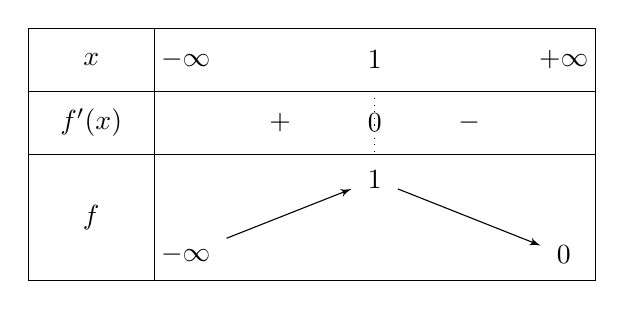
\begin{tikzpicture}[scale=0.8]
   \tkzTabInit{$x$ / 1 , $f'(x)$ / 1, $f$ / 2}{$-\infty$, $1$, $+\infty$}
   \tkzTabLine{, +, z,-,  }
   \tkzTabVar{-/$-\infty$,+/$1$,-/$0$}
\end{tikzpicture}
\end{center}


\item On trace l'allure de la courbe $\mathcal{C}_f$ dans un repère orthogonal.


\begin{center}
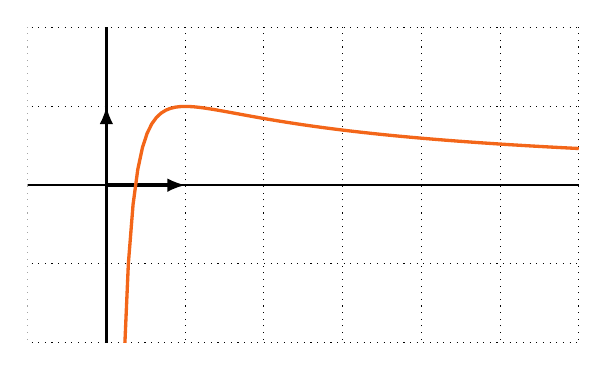
\begin{tikzpicture}[scale=1]
\clip (-1,-2) rectangle (6,2);
\draw [thin, dotted] (-5,-5) grid (6,5);
\draw [thick] (-5,0)--(7,0);
\draw [thick] (0,-5) -- (0,5);
\draw [very thick,->,>=latex] (0,0)--(0,1);
\draw [very thick,->,>=latex] (0,0)--(1,0);
\draw [very thick, ocre,domain=0.1:6,samples=100] plot (\x,{(1+ln(\x))/\x});
\end{tikzpicture}
\end{center}


\item  La fonction $f$ est continue sur $[1;+\infty[$. De plus, $f(1)=1$ et $\displaystyle \lim_{x\to+\infty}f(x)=0$. Ainsi, d'après le théorème des valeurs intermédiaires, il existe un réel $c$ dans $[1;+\infty[$ tel que $f(c)=\dfrac{1}{2}$. De plus, la fonction $f$ étant strictement décroissante sur $[1;+\infty[$, ce réel est unique. A l'aide de la calculatrice, on trouve $x \simeq 5,36$.

\item  Si $m \leqslant 0$, l'équation $f(x)=m$ possède une unique solution sur $]0;+\infty[$.

Si $0 < m < 1$, cette équation possède deux solutions. Si $m=1$, il n'y a qu'une solution. 

Enfin, si $m>1$, l'équation $f(x)=m$ n'a aucune solution.

\end{enumerate}
\end{solution}




\begin{exercise}[topic=log03] Pour tout réel $x>0$, on pose $f(x)=(\ln(x))^2$.
On note $\mathcal{C}_f$ la courbe représentative de $f$ dans un repère orthogonal. Attention, $(\ln(x))^2 \neq \ln(x^2)$ !
\begin{enumerate}
\item Résoudre l'équation $f(x)=1$ sur $]0;+\infty[$.
\item Déterminer les limites de $f$ en $0^+$ et en $+\infty$.
\item Construire le tableau de variations de la fonction $f$ sur $]0;+\infty[$. 
\item Tracer l'allure de la courbe $\mathcal{C}_f$ dans un repère orthogonal.
\item Soit $m \in \mathbb{R}$. Déterminer, selon la valeur du réel $m$, le nombre de solutions de l'équation $f(x)=m$.
\end{enumerate}
\end{exercise}

\begin{solution}\hspace{0pt}
\begin{enumerate}
\item Soit $x>0$
\[ f(x)=1 \Leftrightarrow (\ln(x))^2 = 1 \Leftrightarrow \ln(x)=1 \text{ OU } \ln(x)=-1 \Leftrightarrow x=e \text{ OU } x = \dfrac{1}{e}.\]
\item On a $\displaystyle\lim_{x\to 0^+}\ln(x)=-\infty$ et donc, par produit, $\displaystyle\lim_{x\to 0^+}f(x)=+\infty$. Par ailleurs, $\displaystyle\lim_{x\to +\infty}\ln(x)=+\infty$ et donc $\displaystyle\lim_{x\to +\infty}f(x)=+\infty$.
\item $f$ est dérivable sur $]0;+\infty[$ et pour tout réel $x>0$, $f'(x)= 2 \times \ln(x) \times \dfrac{1}{x} = \dfrac{2\ln(x)}{x}$, qui est du signe de $\ln(x)$.
\begin{center}
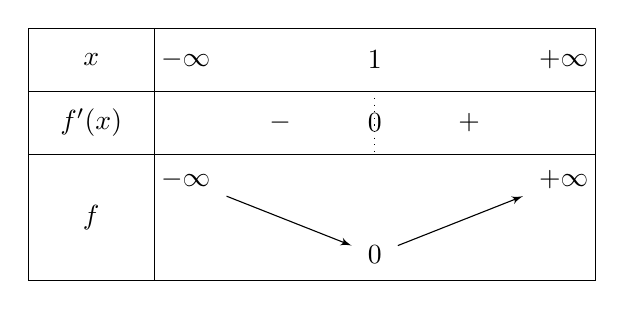
\begin{tikzpicture}[scale=0.8]
   \tkzTabInit{$x$ / 1 , $f'(x)$ / 1, $f$ / 2}{$-\infty$, $1$, $+\infty$}
   \tkzTabLine{, -, z,+,  }
   \tkzTabVar{+/$-\infty$,-/$0$,+/$+\infty$}
\end{tikzpicture}
\end{center}
\item On trace l'allure de la courbe $\mathcal{C}_f$ dans un repère orthogonal.

\begin{center}
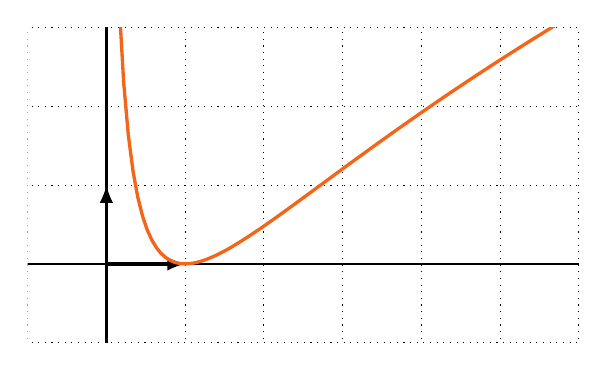
\begin{tikzpicture}[scale=1]
\clip (-1,-1) rectangle (6,3);
\draw [thin, dotted] (-5,-5) grid (6,5);
\draw [thick] (-5,0)--(7,0);
\draw [thick] (0,-5) -- (0,5);
\draw [very thick,->,>=latex] (0,0)--(0,1);
\draw [very thick,->,>=latex] (0,0)--(1,0);
\draw [very thick, ocre,domain=0.1:6,samples=100] plot (\x,{ln(\x)*ln(\x)});
\end{tikzpicture}
\end{center}

\item Si $m < 0$, l'équation $f(x)=m$ n'admet aucune solution sur $]0;+\infty[$.

Si $m=0$, cette équation possède une unique solution. Si $m>0$, il y a deux solutions.

\end{enumerate}
\end{solution}




\begin{exercise}[topic=log03]
Pour tout réel $x$, on pose $f(x)=\ln(x^2-2x+3)$.
\begin{enumerate}
\item Justifier que la fonction $f$ est bien définie sur $\mathbb{R}$.
\item Justifier que $f$ est dérivable sur $\mathbb{R}$ puis calculer sa dérivée $f'$.
\item Construire le tableau de variations de $f$ sur $\mathbb{R}$ en incluant les limites en $-\infty$ et en $+\infty$ de la fonction $f$.
\end{enumerate}
\end{exercise}

\begin{solution}Le discriminant du polynôme $x^2-2x+3$ vaut $-8$ qui est négatif. Ainsi, pour tout réel $x$, $x^2-2x+3>0$. $f$ est bien définie sur $\mathbb{R}$.

La fonction $x\mapsto x^2-2x+3$ est strictement positive et dérivable sur $\mathbb{R}$. $f$ est donc dérivable sur $\mathbb{R}$ et pour tout réel $x$, $f'(x)=\dfrac{2x-2}{x^2-2x+3}$.

Puisque pour tout réel $x$, $x^2-2x+3>0$, $f'(x)$ est du signe de $2x-2$.

\begin{center}
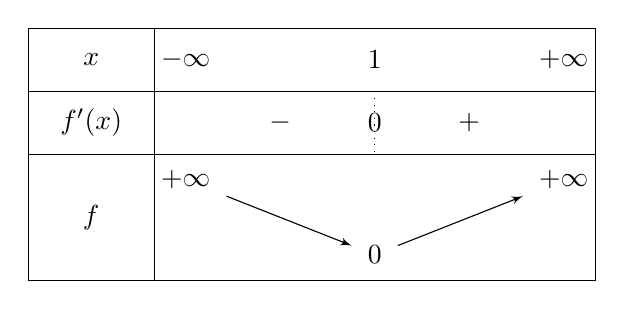
\begin{tikzpicture}[scale=0.8]
   \tkzTabInit{$x$ / 1 , $f'(x)$/1, $f$/2}{$-\infty$, $1$, $+\infty$}
   \tkzTabLine{,- ,z, +,  }
   \tkzTabVar{+/$+\infty$,-/$0$,+/$+\infty$}
\end{tikzpicture}
\end{center}\end{solution}






\begin{exercise}[topic=log03]A l'aide du logarithme, déterminer le plus petit entier naturel $n$ vérifiant les conditions suivantes.
\vspace{-0.5cm}
\begin{center}
\begin{tabularx}{0.9\linewidth}{XXX}
\textbf{a.} $2^n \geqslant 40000$ & \textbf{b.} $1.01^n \geqslant 2$ & \textbf{c.} $0.7^n \leqslant 10^{-3}$\\
\textbf{d.} $121 \times 0,97^{2n+1} \leqslant 1$ &\textbf{e.}  $3 \times 1,1^n -150 \geqslant 365$ & \textbf{f.} $ 10^{12}\times 2^{-n} \leqslant 0,1$
\end{tabularx}
\end{center}\end{exercise}

\begin{solution}\textbf{a.}  Par croissance du logarithme népérien sur $]0;+\infty[$, $2^n \geqslant 40000$ si et seulement si $\ln(2^n) \geqslant \ln(40000)$ soit $n\ln(2) \geqslant \ln(40000)$ et, $\ln(2)$ étant positif, $n \geqslant \dfrac{\ln(40000)}{\ln(2)}$. L'entier recherché est 16.
\vskip5pt
\textbf{b.}  Par croissance du logarithme népérien sur $]0;+\infty[$, $1.01^n \geqslant 2$ si et seulement si $\ln(1.01^n) \geqslant \ln(2)$ soit $n\ln(1.01) \geqslant \ln(2)$ et, $\ln(1.01)$ étant positif, $n \geqslant \dfrac{\ln(2)}{\ln(1.01)}$. L'entier recherché est 70.
\vskip5pt
\textbf{c.}  Par croissance du logarithme népérien sur $]0;+\infty[$, $0.7^n \leqslant 10^{-3}$ si et seulement si $\ln(0.7^n) \leqslant \ln(10^{-3})$ soit $n\ln(0.7) \leqslant -3\ln(10)$ et, $\ln(0.7)$ étant négatif, $n \geqslant \dfrac{-3\ln(10)}{\ln(0.7)}$. L'entier recherché est 20.
\vskip5pt
\textbf{d.} \(121 \times 0,97^{2n+1} \leqslant 1\) si et seulement si \(0,97^{2n+1} \leqslant \dfrac{1}{121}\). Par croissance du logarithme népérien sur \(]0;+\infty[\), ceci équivaut à \((2n+1)\ln(0.97) \leqslant -\ln(121)\). En divisant par \(\ln(0.97)\) qui est négatif, on obtient \(2n+1\geqslant -\dfrac{\ln(121)}{\ln(0.97)}\) et donc \(n \geqslant \dfrac{1}{2}\left(-\dfrac{\ln(121)}{\ln(0.97)}-1\right)\). L'entier recherché est 79.
\vskip5pt
\textbf{e.} \(3 \times 1,1^n -150 \geqslant 365\) si et seulement si \(1.1^n \geqslant \dfrac{515}{3}\). Par croissance du logarithme népérien sur \(]0;+\infty[\), ceci équivaut à \(n\ln(1.1)\geqslant \ln(515)-\ln(3)\) et donc \(n\geqslant \dfrac{\ln(515)-\ln(3)}{\ln(1.1)}\). L'entier recherché est 54.
\vskip5pt
\textbf{f.}  \( 10^{12}\times 2^{-n} \leqslant 0,1\) équivaut à \(2^{-n} \leqslant 10^{-13}\). Par croissance du logarithme népérien sur \(]0;+\infty[\), ceci équivaut à \(-n\ln(2) \leqslant -13\ln(10)\) et donc \(n\geqslant \dfrac{13\ln(10)}{\ln(2)}\). L'entier recherché est 44.
\end{solution}



\begin{exercise}[topic=log03]Résoudre l'inéquation $(e^{2x}-3)(\ln(x)-1)<0$ sur $\mathbb{R}$. On précisera le domaine de définition de cette expression.\end{exercise}

\begin{solution}

L'expression \((e^{2x}-3)(\ln(x)-1)\) existe pour tout réel \(x > 0\). Construisons le tableau de signe de cette expression.


\begin{center}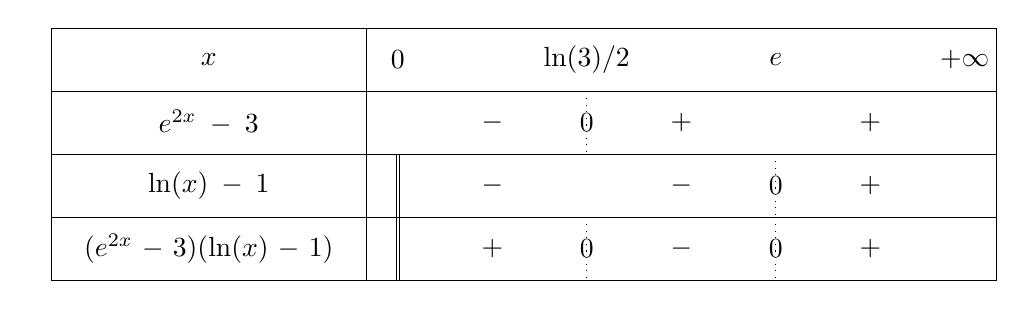
\begin{tikzpicture}[scale=0.8]
\tkzTabInit[lgt=5]{$x$ / 1 , $e^{2x}-3$/1, $\ln(x)-1$/1, $(e^{2x}-3)(\ln(x)-1)$/1 }{$0$, $\ln(3)/2$, $e$,  $+\infty$}
\tkzTabLine{, -,z,+,,+, }
\tkzTabLine{d, -,,-,z,+, }
\tkzTabLine{d, +,z,-,z,+, }
\end{tikzpicture}\end{center}


Ainsi, l'ensemble solution recherché est \(S=\left]0;\dfrac{\ln(3)}{2}\right[ \cup \left]e;+\infty\right[\).

\end{solution}




\begin{exercise}[topic=log03]On considère la suite $(u_n)$ définie par $u_0=5$ et, pour tout entier naturel $n$ par $u_n=\dfrac{7}{8}u_n+1$. Pour tout entier naturel $n$, on pose alors $a_n=u_n-8$.
\begin{enumerate}
\item Montrer que la suite $(a_n)$ est géométrique de raison $\dfrac{7}{8}$ et déterminer son premier terme.
\item En déduire que pour tout entier naturel $n$, $u_n=8-3\times\left(\dfrac{7}{8}\right)^n$. Que vaut $\displaystyle\lim_{n \to +\infty}u_n$ ?
\item Déterminer le plus petit entier $n$ à partir duquel $u_n \geqslant 7,999$.
\end{enumerate}\end{exercise}

\begin{solution}\hspace{0pt}

\begin{enumerate}\item Pour tout entier naturel \(n\), $a_{n+1}=u_{n+1}-8=\dfrac{7}{8}u_n+1-8=\dfrac{7}{8}(a_n+8)-7=\dfrac{7}{8}a_n$.\\
La suite \((a_n)\) est donc géométrique, de raison \(\dfrac{7}{8}\) et de premier terme \(a_0=u_0-8=-3\).

\item Ainsi, pour tout entier naturel \(n\), \(a_n=-3 \left(\dfrac{7}{8}\right)^n\) et \(u_n=a_n+8=8-3\times\left(\dfrac{7}{8}\right)^n\).

\item  Soit \(n\) un entier naturel. On a \(u_n \geqslant 7,999\) si et seulement si \(8-3\times\left(\dfrac{7}{8}\right)^n\geqslant 7.999\), soit \(\left(\dfrac{7}{8}\right)^n \leqslant \dfrac{0.001}{3}\). \\ Par croissance du logarithme népérien sur \(]0;+\infty[\), ceci équivaut à \(n\ln\left(\dfrac{7}{8}\right) \leqslant \ln\left(\dfrac{0.001}{3}\right)\) et donc, en divisant par \(\ln\left(\dfrac{7}{8}\right)\) qui est négatif,  \(n \geqslant \dfrac{\ln\left(\frac{0.001}{3}\right)}{\ln\left(\frac{7}{8}\right)}\). L'entier recherché est 60.\end{enumerate}
\end{solution}



\begin{exercise}[topic=log03]La population d'une ville augmente de 3\% chaque année. Après combien d'années cette population aura-t-elle doublé ?\end{exercise}

\begin{solution}

Soit \(n\) un entier naturel. Après \(n\) années, la population de cette ville a été multipliée par \(1.03^n\). On cherche donc à résoudre l'équation \(1.03^n \geqslant 2\), ce qui équivaut à \(n\geqslant \dfrac{\ln(2)}{\ln(1.03)}\). L'entier recherché est 24 : la population aura doublé en 24 ans.
\end{solution}






\begin{exercise}[topic=log03]Pour tout réel $x$, on pose $f(x)=\ln(1+e^x)$. Cette fonction, utilisée en intelligence artificielle, est appelée fonction SoftPlus.
\begin{enumerate}
\item Justifier que la fonction $f$ est bien définie sur $\mathbb{R}$.
\item Justifier que $f$ est dérivable sur $\mathbb{R}$ puis calculer sa dérivée $f'$.
\item Construire le tableau de variations de $f$ sur $\mathbb{R}$ en incluant les limites en $-\infty$ et en $+\infty$ de la fonction $f$.
\item Pour tout réel $x$, on pose $g(x)=f(x)-x$.
\begin{enumerate}
\item Montrer que pour tout réel $x$, $g(x)=\ln(1+e^{-x})$.
\item En déduire $\displaystyle\lim_{x\to +\infty}g(x)=0$. 
\end{enumerate}
\item \begin{enumerate}
\item Dresser le tableau de variations de $g$ sur $\mathbb{R}$ en incluant les limites en $-\infty$ et $+\infty$.
\item En déduire que pour tout réel $x$, $f(x)\geqslant x$.
\end{enumerate}

\item Construire l'allure de la courbe de $f$ dans un repère orthonormé.
\end{enumerate}\end{exercise}

\begin{solution}\hspace{0pt}

\begin{enumerate}\item Pour tout réel \(x\), \(e^x >0\) et donc \(1+e^x>0\). \(f\) est donc bien définie sur \(\mathbb{R}\).
	\item \(f\) est dérivable comme composition de fonctions dérivables. Pour tout réel \(x\), \(f'(x)=\dfrac{e^x}{1+e^x}\).
	\item On a \(\displaystyle\lim_{x \to + \infty}(1+e^x)=+\infty\) et \(\displaystyle\lim_{x \to - \infty}(1+e^x)=1\). Ainsi, \(\displaystyle\lim_{x \to + \infty}f(x)=+\infty\) et \(\displaystyle\lim_{x \to - \infty}f(x)=\ln(1)=0\). On obtient alors le tableau de variations suivant.


\begin{center}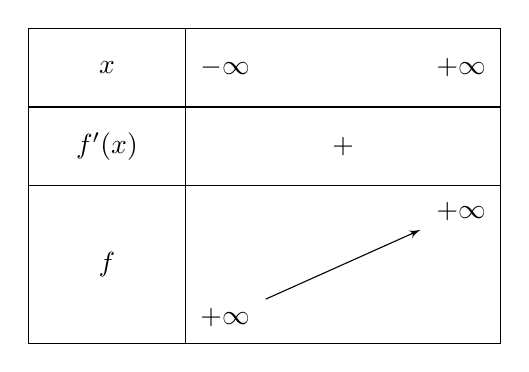
\begin{tikzpicture}[scale=1]
\tkzTabInit{$x$ / 1 , $f'(x)$/1, $f$/2}{$-\infty$,  $+\infty$}
\tkzTabLine{, +, }
\tkzTabVar{-/$+\infty$,+/$+\infty$}
\end{tikzpicture}\end{center}

\item \begin{enumerate}\item Pour tout réel \(x\), \[g(x)=f(x)-x=\ln(1+e^x)-\ln(e^x)=\ln\left(\dfrac{1+e^x}{e^x}\right)=\ln(e^{-x}+1).\]
	\item Pour tout réel \(x\), \(1+e^{-x}>1\) et donc \(\ln(1+e^{-x})>0\), par croissance du logarithme népérien sur \([1;+\infty[\). Il en vient que pour tout réel \(x\), \(g(x)>0\), soit \(f(x)-x>0\) et donc \(f(x)>x\).
	\item Puisque \(\displaystyle\lim_{x\to +\infty}(1+e^{-x})=1\), on a \(\displaystyle\lim_{x\to +\infty}g(x)=0\). La courbe de \(f\) se rapproche de la droite d'équation \(y=x\) au voisinage de \(+\infty\).\end{enumerate}
	\item 

\begin{center}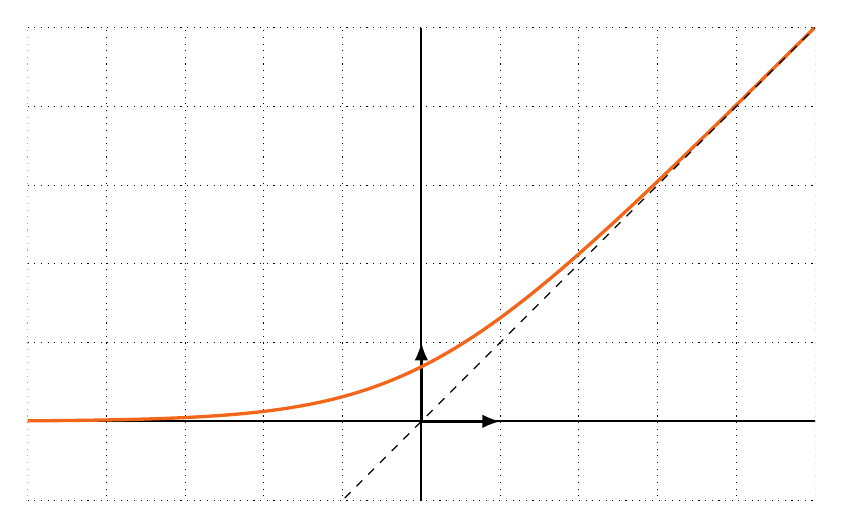
\begin{tikzpicture}[scale=1]
\clip (-5,-1) rectangle (5,5);
\draw [thin, dotted] (-5,-5) grid (6,5);
\draw [thick] (-5,0)--(7,0);
\draw [thick] (0,-5) -- (0,5);
\draw [very thick,->,>=latex] (0,0)--(0,1);
\draw [very thick,->,>=latex] (0,0)--(1,0);
\draw [very thick, ocre,domain=-5:6,samples=100] plot (\x,{ln(1+exp(\x)});
\draw [dashed,domain=-5:6,samples=100] plot (\x,{\x});
\end{tikzpicture}\end{center}
\end{enumerate}


\end{solution}




\begin{exercise}[topic=log03]On considère la fonction $f$ définie pour tout réel $x>0$ par $f(x)=\sqrt{x}+\ln(x)$. 
\begin{enumerate}
\item Déterminer les limites de $f(x)$ lorsque $x$ tend vers 0 et lorsque $x$ tend vers $+\infty$.
\item On admet que $f$ est dérivable sur $]0;+\infty[$. Montrer que pour tout réel $x>0$, $f'(x)=\dfrac{\sqrt{x}+2}{2x}$.
\item Quel est le sens de variations de la fonction $f$ ?
\item En déduire qu'il existe un unique réel $\alpha>0$ tel que $\sqrt{\alpha}=-\ln(\alpha)$. Donner une valeur approchée de $\alpha$ à $10^{-2}$ près.\end{enumerate}\end{exercise}

\begin{solution}\hspace{0pt}

\begin{enumerate}
\item Par somme de limites, $\displaystyle\lim_{x\to 0^+}f(x)=-\infty$ et $\displaystyle\lim_{x\to+\infty}f(x)=+\infty$.
\item Pour tout réel $x>0$, $f'(x)=\dfrac{1}{2\sqrt{x}}+\dfrac{1}{x}=\dfrac{\sqrt{x}}{2x}+\dfrac{2}{2x}=\dfrac{\sqrt{x}+2}{2x}$.
\item Pour tout réel $x>0$, $f'(x)>0$. $f$ est donc strictement croissante sur $]0;+\infty[$.
\item $f$ est continue sur $]0;+\infty[$. De plus, $\displaystyle\lim_{x\to 0^+}f(x)=-\infty$ et $\displaystyle\lim_{x\to+\infty}f(x)=+\infty$. D'après le théorème des valeurs intermédiaires, il existe un réel $\alpha \in ]0;+\infty[$ tel que $f(\alpha)=0$, c'est-à-dire $\sqrt{\alpha}+\ln(\alpha)=0$ ou encore $\sqrt{\alpha}=-\ln(\alpha)$. A l'aide de la calculatrice, on trouve $\alpha \simeq 0.49$.
\end{enumerate}

\end{solution}




\begin{exercise}[topic=log03]Faire l'étude complète de la fonction $x\mapsto \ln(e^x-x)$ sur $\mathbb{R}$ puis tracer l'allure de la courbe représentative de cette fonction dans un repère orthogonal.\newpage \end{exercise}

\begin{solution}Pour tout réel $x$, on pose $u(x)=e^x-x$. $u$ est dérivable sur $\mathbb{R}$ et pour tout réel $x$, $u'(x)=e^x-1$. On en déduit le tableau de variations de $u$.
	

\begin{center}
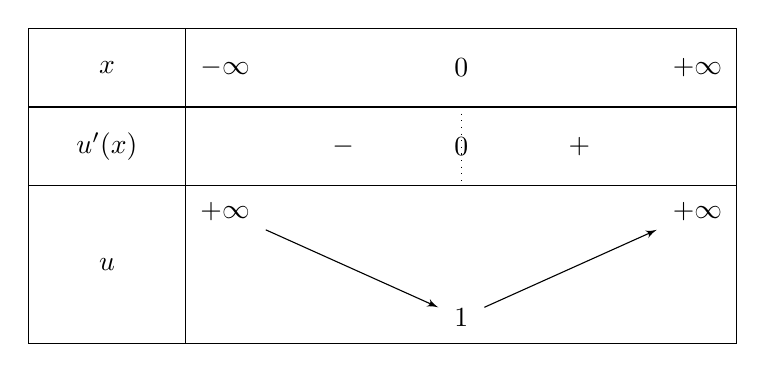
\begin{tikzpicture}[scale=1]
   \tkzTabInit{$x$ / 1 , $u'(x)$/1, $u$/2}{$-\infty$, $0$, $+\infty$}
   \tkzTabLine{,- ,z, +,  }
   \tkzTabVar{+/$+\infty$,-/$1$,+/$+\infty$}
\end{tikzpicture}
\end{center}


En particulier, pour tout réel $x$, $e^x-x\geqslant 1$ et donc $e^x-x>0$. $f$ est donc définie sur $\mathbb{R}$. $f$ est également dérivable sur $\mathbb{R}$ et pour tout réel $x$, $f'(x)=\dfrac{e^x-1}{e^x-x}$. Les variations de $f$ sont les mêmes que les variations de $u$. On a donc le tableau de variations suivant.

\begin{center}
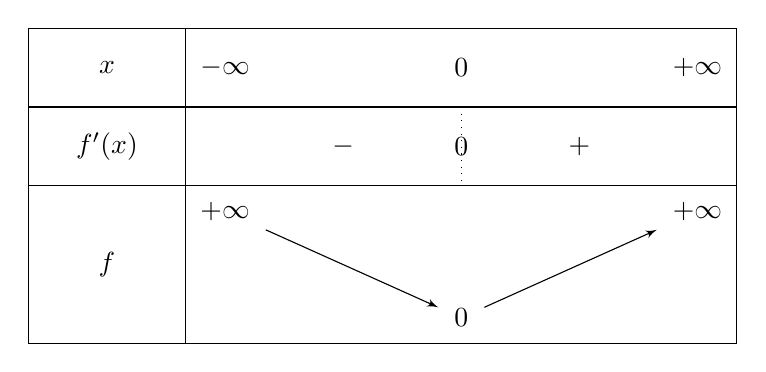
\begin{tikzpicture}[scale=1]
   \tkzTabInit{$x$ / 1 , $f'(x)$/1, $f$/2}{$-\infty$, $0$, $+\infty$}
   \tkzTabLine{,- ,z, +,  }
   \tkzTabVar{+/$+\infty$,-/$0$,+/$+\infty$}
\end{tikzpicture}
\end{center}

On peut alors tracer l'allure de la courbe de $f$.

\begin{center}
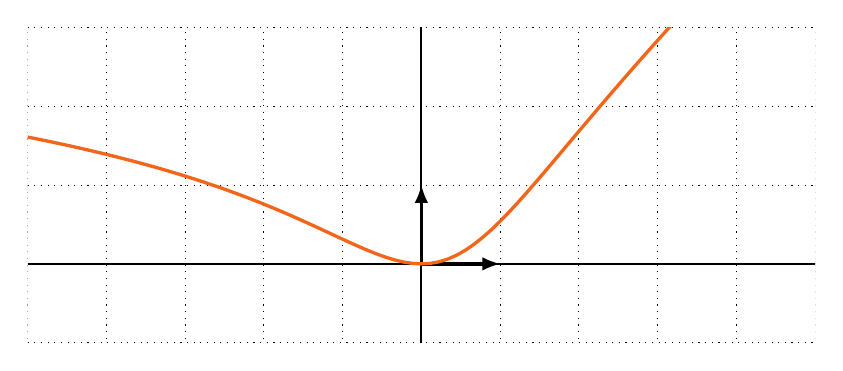
\begin{tikzpicture}[scale=1]
\clip (-5,-1) rectangle (5,3);
\draw [thin, dotted] (-5,-5) grid (6,5);
\draw [thick] (-5,0)--(7,0);
\draw [thick] (0,-5) -- (0,5);
\draw [very thick,->,>=latex] (0,0)--(0,1);
\draw [very thick,->,>=latex] (0,0)--(1,0);
\draw [very thick, ocre,domain=-5:6,samples=100] plot (\x,{ln(exp(\x)-\x)});
\end{tikzpicture}
\end{center}

\end{solution}

\printcollection{log03}

\section*{Exercices de synthèse}

\begin{exercise}[topic=log04, subtitle={(Amérique du Nord 2021)}] Dans le plan muni d'un repère, on considère ci-dessous la courbe $C_f$
représentative d'une fonction $f$, deux fois dérivable sur l'intervalle $]0;+\infty[$. La courbe $C_f$ admet une tangente horizontale $T$ au point $A(1;4)$.

\begin{center}
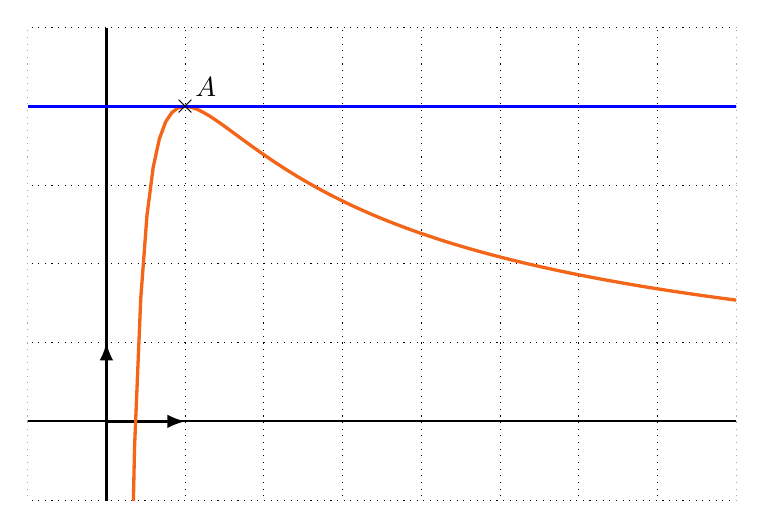
\begin{tikzpicture}[scale=1]
\clip (-1,-1) rectangle (8,5);
\draw [thin, dotted] (-5,-5) grid (8,5);
\draw [thick] (-5,0)--(8,0);
\draw [thick] (0,-5) -- (0,5);
\draw [very thick,->,>=latex] (0,0)--(0,1);
\draw [very thick,->,>=latex] (0,0)--(1,0);
\draw [very thick, ocre,domain=0.2:8,samples=100] plot (\x,{(4+4*ln(\x))/\x});
\draw [thick, blue,domain=-1:8,samples=100] plot (\x,{4});
\draw [thick] (1,4) node[above right] {$A$};
\draw [thick] (1,4) node {$\times$};
\draw [thick, blue] (6,8) node[above] {$T$};
\end{tikzpicture}
\end{center}

\begin{enumerate}
\item Préciser les valeurs de $f(1)$ et $f'(1)$.
\end{enumerate}
On admet que la fonction $f$ est définie pour tout réel $x$ de l'intervalle $]0;+\infty [$ par
\[f(x)=\dfrac{a+b\ln(x)}{x} \quad \text{où } a \text{ et }b\text{ sont des réels fixés.}\]
\begin{enumerate}
\setcounter{enumi}{1}
\item Démontrer que pour tout réel $x$ strictement positif, on a
\[f'(x)=\dfrac{b-a-b\ln(x)}{x^2}.\]
\item En déduire les valeurs de $a$ et de $b$.
\end{enumerate}
Dans la suite de l'exercice, on admet que la fonction $f$ est définie pour tout réel $x$ de l'intervalle $]0,+\infty[$ par
\[f(x)=\dfrac{4+4\ln(x)}{x}.\]
\begin{enumerate}
\setcounter{enumi}{3}
\item Déterminer les limites de $f$ en $0$ et en $+\infty$.
\item Déterminer le tableau de variations de $f$ sur $]0;+\infty[$.
\item Démontrer que, pour tout réel $x$ strictement positif,
\[f''(x)=\dfrac{-4+8\ln(x)}{x^3}.\]
\item Construire le tableau de signes de $f''$. Nous verrons dans un prochain chapitre que le signe de $f''$ nous permet de déterminer la convexité de la fonction $f$.
\end{enumerate}
\newpage
\end{exercise}

\begin{solution}\hspace{0pt}

\begin{enumerate}\item D'après le graphique, on a \(f(1)=4\) et \(f'(1)=0\).
	\item Pour tout réel \(x\) strictement positif,
	\[f'(x)=\dfrac{\frac{b}{x} \times x - (a+b\ln(x)) \times 1}{x^2}=\dfrac{b-a-b\ln(x)}{x^2}.\]
	\item D'une part, \(f(1)=4\) d'après le graphique. Or, en utilisant la formule, on a \(f(1)=\dfrac{a+b\ln(1)}{1}=a\). Ainsi, \(a=4\). Par ailleurs, \(f'(1)=0\) d'après le graphique, et \(f'(1)=\dfrac{b-4-b\ln(1)}{1^2}=b-4\) en utilisant la formule. Il en vient que \(b-4=0\) et donc \(b=4\).
	\item On a \(\displaystyle\lim_{x \to 0^+}(4+4\ln(x))=-\infty\) et donc \(\displaystyle\lim_{x \to 0^+}(f(x))=-\infty\). Par ailleurs, pour tout réel \(x\) strictement positif, \(f(x)=\dfrac{4}{x}+\dfrac{4\ln(x)}{x}\). Par croissances comparées et somme de limites, \(\displaystyle\lim_{x \to +\infty}(f(x))=0\).
	\item Pour tout \(x>0\), \(f'(x)=\dfrac{-4\ln(x)}{x^2}\) est du signe opposé à celui de \(\ln(x)\).

		
\begin{center}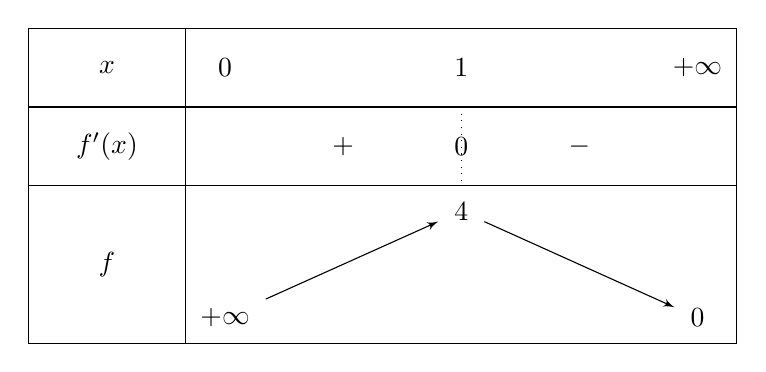
\begin{tikzpicture}[scale=1]
\tkzTabInit{$x$ / 1 , $f'(x)$/1, $f$/2}{$0$, $1$,  $+\infty$}
\tkzTabLine{, +,z,-, }
\tkzTabVar{-/$+\infty$,+/$4$,-/$0$}
\end{tikzpicture}\end{center}


\item Pour tout réel $x>0$, $f''(x)=\dfrac{-\dfrac{4}{x} \times x^2 - (-4\ln(x))\times 2x}{(x^2)^2}=\dfrac{x(-4+8\ln(x))}{x^4}=\dfrac{-4+8\ln(x)}{x^3}$.

\item Pour tout $x>0$, on a $x^3>0$ et $-4+8\ln(x)>0$ si et seulement si $\ln(x) > \dfrac{1}{2}$ soit $x>\sqrt{e}$.

\begin{center}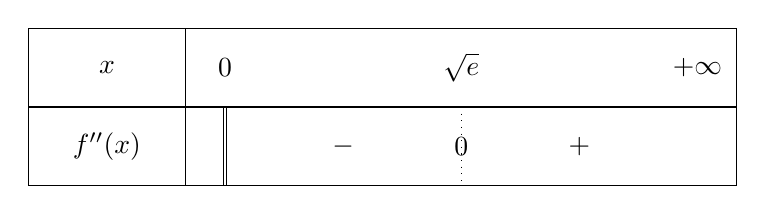
\begin{tikzpicture}[scale=1]
\tkzTabInit{$x$ / 1 , $f''(x)$/1}{$0$, $\sqrt{e}$,  $+\infty$}
\tkzTabLine{d, -,z,+, }
\end{tikzpicture}\end{center}

\end{enumerate}
\end{solution}

%
\begin{exercise}[topic=log04, subtitle={(Métropole 2022)}]On considère la fonction $f$ définie sur $]0;+\infty[$ par $f(x)=x-x\ln(x)$ où $\ln$ désigne la fonction logarithme népérien.

\textbf{Partie A}

\begin{enumerate}
\item Déterminer la limite de $f(x)$ quand $x$ tend vers 0 et quand $x$ tend vers $+\infty$.
\item On admet que la fonction $f$ est dérivable sur $]0;+\infty[$ et on note $f'$ sa fonction dérivée.
\begin{enumerate}
\item Démontrer que pour tout réel $x>0$, $f'(x)=-\ln(x)$.
\item En déduire les variations de la fonction $f$ sur $]0;+\infty[$.
\end{enumerate}
\item Résoudre l'équation $f(x)=x$ sur $]0;+\infty[$.
\end{enumerate}

\textbf{Partie B}

Dans cette partie, on pourra utiliser avec profit certains résultats de la partie A.\\
On considère la suite $(un_)$ définie par
\[\left\{\renewcommand{\arraystretch}{1.2} \begin{array}{l}u_0=0.5 \\ u_{n+1}=u_n-u_n\ln(u_n) \text{ pour tout entier naturel }n

\end{array}\right.\]
Ainsi, pour tout entier naturel $n$, $u_{n+1}=f(u_n)$.
\begin{enumerate}
\item On rappelle que la fonction $f$ est croissante sur $[0,5;1]$.\\
Démontrer par récurrence que pour tout entier naturel $n$, $0.5\leqslant u_n \leqslant u_{n+1} \leqslant 1$.
\item \begin{enumerate}
\item Montrer que la suite $(u_n)$ converge.
\item On note $\ell$ la limite de la suite $(u_n)$. Déterminer la valeur de $\ell$.
\end{enumerate}
\end{enumerate}

\textbf{Partie C}

Pour un nombre $k$ quelconque, on considère la fonction $f_k$ définie sur $]0;+\infty[$ par $f_k(x)=kx-x\ln(x)$.
\begin{enumerate}
\item Pour tout nombre réel $k$, montrer que $f_k$ admet un maximum $y_k$ atteint en $x_k=e^{k-1}$.
\item Montrer que, pour tout nombre réel $k$, $x_k=y_x$.
\end{enumerate}\end{exercise}

\begin{solution}\hspace{0pt}

\textbf{Partie A}

\begin{enumerate}
 \item Par croissances, comparées, $\displaystyle\lim_{x \to 0^+} x\ln(x)=0$. Ainsi, $\displaystyle\lim_{x\to 0^+}f(x)=0$.
 \item Pour tout réel $x>0$, $f(x)=x(1-\ln(x))$. Or, $\displaystyle\lim_{x\to+\infty}x=+\infty$ et $\displaystyle\lim_{x\to +\infty}(1-\ln(x))=-\infty$. Par produit, $\displaystyle\lim_{x\to +\infty}f(x)=-\infty$.
 \item \begin{enumerate}
 \item Pour tout réel $x>0$, $f'(x)= 1-\left(1\times \ln(x)+x \times \dfrac{1}{x}\right)=1-\ln(x)+1=-\ln(x)$.
 \item On en déduit le tableau de signes de $f'$ et le tableau de variations de $f$.
 
 \begin{center}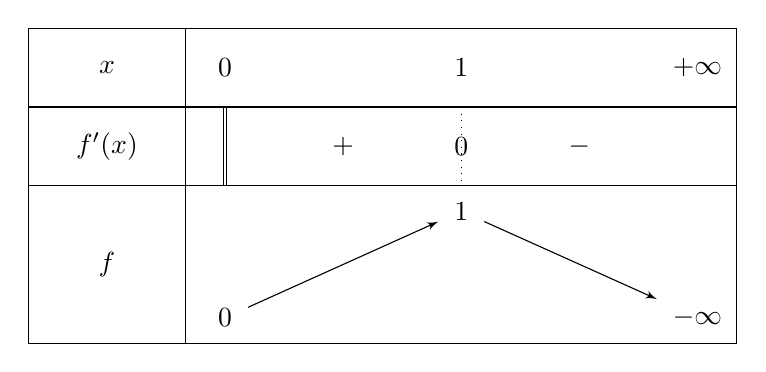
\begin{tikzpicture}[scale=1]
   \tkzTabInit{$x$ / 1 , $f'(x)$ / 1, $f$ / 2}{$0$, $1$, $+\infty$}
   \tkzTabLine{d, +, z,-,  }
   \tkzTabVar{-/$0$,+/$1$,-/$-\infty$}
\end{tikzpicture}\end{center}

 \end{enumerate}
\item On a $f(x)=x$ si et seulement si $x-x\ln(x)=x$ soit $-x\ln(x)=0$. Puisque $x>0$, l'unique solution de cette équation est $x=1$.
\end{enumerate}

\textbf{Partie B}

\begin{enumerate}
\item Pour tout entier naturel $n$, on considère la proposition $P(n)$ : « $0.5\leqslant u_n \leqslant u_{n+1} \leqslant 1$ ».
\begin{itemize}
\item On a $u_0=0.5$ et $u_1=0.5-0.5\ln(0.5)\simeq 0.84$. On a bien  $0.5\leqslant u_0 \leqslant u_{1} \leqslant 1$. $P(0)$ est vraie.
\item Soit $n$ un entier naturel tel que $P(n)$ est vraie. On a alors  $0.5\leqslant u_n \leqslant u_{n+1} \leqslant 1$. Puisque la fonction $f$ est croissante sur $[0.5;1]$ on a alors $f(0.5)\leqslant f(u_n) \leqslant f(u_{n+1}) \leqslant f(1)$. Or, $f(0.5)\geqslant 0.5$ et $f(1)=1$. Ainsi, on a $0.5\leqslant u_{n+1} \leqslant u_{n+2} \leqslant 1$. $P(n+1)$ est donc vraie.
\item Par récurrence, $P(n)$ est vraie pour tout entier naturel $n$.
\end{itemize}
\item \begin{enumerate}
\item D'après la question précédente, la suite $(u_n)$ est croissante et majorée, elle est donc convergente.
 \item Puisque la fonction $f$ est continue sur $[0.5;1]$ et que pour tout entier naturel $n$, $u_n \in [0.5;1]$, alors $f(\ell)=\ell$. Or, l'unique solution de cette équation sur cet intervalle est 1. Ainsi, $\ell=1$.
\end{enumerate}
\end{enumerate}

\textbf{Partie C}

Pour tout réel $k$, pour tout réel $x$, $f_k$ est dérivable sur $]0;+\infty[$ et $f_k'(x)=k-\left(1 \times \ln(x) + x \times \frac{1}{x}\right)=k-1-\ln(x)$.

Or, $f_k'(x)\leqslant 0$ si et seulement si $k-1-\ln(x)\leqslant 0$ si et seulement si $k-1 \leqslant \ln(x)$ si et seulement si $x\geqslant e^{k-1}$

\begin{center}
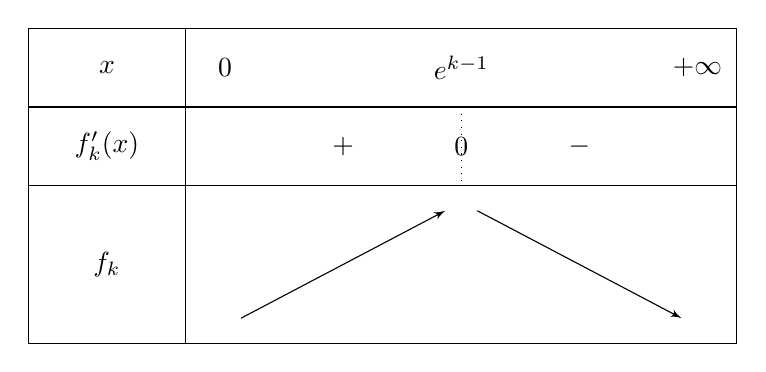
\begin{tikzpicture}[scale=1]
   \tkzTabInit{$x$ / 1 , $f_k'(x)$/1, $f_k$/2}{$0$, $e^{k-1}$, $+\infty$}
   \tkzTabLine{,+ ,z, -,  }
   \tkzTabVar{-/$ $,+/$ $,-/$ $}
\end{tikzpicture}
\end{center}

Ainsi, $f_k$ admet un maximum en $x_k=e^{k-1}$.

 Par ailleurs, $f_k(x_k)=ke^{k-1}-e^{k-1} \times \ln(e^{k-1})=ke^{k-1}-(k-1)e^{k-1}=e^{k-1}$.\end{solution}
 
 
 

\begin{exercise}[topic=log04, subtitle={(Centres étrangers 2021)}]Dans un pays, une maladie touche la population avec une probabilité de $0,05$.

On possède un test de dépistage de cette maladie. On considère un échantillon de $n$ personnes ($n>20$) prises au hasard dans la population assimilé à un tirage avec remise.

On teste l'échantillon suivant cette méthode : on mélange le sang de ces $n$ individus, on teste le mélange. Si le test est positif, on effectue une analyse individuelle de chaque personne.

Soit $X_n$ la variable aléatoire qui donne le nombre d'analyses effectuées.
\begin{enumerate}
\item Justifier que $X_n$ prend les valeurs 1 et $(n +1)$.
\item Justifier que $\mathbb{P}(X_n=1)=0.95^n$.
\item Que représente l'espérance de $X_n$ dans ce cadre ? Montrer que $E(X_n)=n+1-n \times 0,95^n$.

\item On considère la fonction $f$ définie sur $[20 ; +\infty[$ par $f (x) = \ln(x)+ x \ln(0,95)$.
\begin{enumerate}
\item Montrer que $f$ est décroissante sur $[20 ; +\infty[$ et calculer $\displaystyle\lim_{x \to + \infty}f(x)$.
\item Montrer que l'équation  $f (x) = 0$ admet une unique solution a sur $[20 ; +\infty[$.
Donner un encadrement à 0,1 près de cette solution.
\item En déduire le signe de $f$ sur $[20 ; +\infty[$. \end{enumerate}
\item On cherche à comparer deux types de dépistages.
La première méthode est décrite dans cet exercice, la seconde, plus classique, consiste à tester tous les individus.
La première méthode permet de diminuer le nombre d'analyses dès que $E (X_n) < n$.
En utilisant les questions précédentes, montrer que la première méthode diminue le nombre d'analyses pour des échantillons comportant 87 personnes maximum.\end{enumerate}\end{exercise}

\begin{solution} \hspace{0pt}

\begin{enumerate}
\item Si le test est négatif on aura fait un test : dans ce cas, on a $X_n = 1$. Sinon, on aura fait un test joint puis $n$ tests individuels : on aura alors $X_n=n+1$.
\item $\mathbb{P}(X_n = 1)$ est la probabilité que l'on ne fasse qu'un test : cela signifie que le test des $n$ personnes est négatif et donc qu'elles ne sont pas malades. La probabilité qu'une personne au hasard soit malade est égale à 0.05. La probabilité qu'une personne au hasard soit saine est donc de 0.95. Le tirage étant assimilé à un tirage avec remise, on suppose ceux-ci indépendants. La probabilité que les $n$ personnes soient saines vaut donc $0.95^n$.
\item Puisque $X_n$ ne peut prendre que les valeurs 1 et $n+1$, on a alors $\mathbb{P}(X_n = n+1)=1-0.95^n$.

Ainsi, $E[X_n]=(n+1) \times \mathbb{P}(X_n=n+1)+1\times \mathbb{P}(X_n = 1)=(n+1)(1-0.95^n)+0.95^n$ et donc $E[X_n]=n+1-n \times 0.95^n$.

Cette espérance représente le nombre moyen d'analyses à effectuer pour un échantillon de $n$ personnes.
\item \begin{enumerate}
\item $f$ est dérivable sur $[20;+\infty[$ et pour tout réel $x$ de cet intervalle, $f'(x)=\dfrac{1}{x}+\ln(0.95)$.

Or, $x \geqslant 20$ et donc $\dfrac{1}{x}\leqslant 0.05$ puis $f'(x)\leqslant 0.05 + \ln(0.95) < 0$. $f$ est strictement décroissante sur $[20;+\infty[$.

Par ailleurs, pour tout réel $x\geqslant 20$, $f(x)=x\left(\dfrac{\ln(x)}{x}+\ln(0.95)\right)$. Or, par croissances comparées, $\displaystyle\lim_{x\to+\infty}\dfrac{\ln(x)}{x}=0$ et donc $\displaystyle\lim_{x\to+\infty}\left(\dfrac{\ln(x)}{x}+\ln(0.95)\right)=\ln(0.95)<0$. 

Par produit, $\displaystyle\lim_{x\to+\infty}f(x)=-\infty$.
\item La fonction $f$ est continue sur $[20;+\infty[$. On a $f(20)\simeq 1.97$ et  $\displaystyle\lim_{x\to+\infty}f(x)=-\infty$. D'après le théorème des valeurs intermédiaires, il existe un réel $\alpha \geqslant 20$ tel que $f(\alpha)=0$. De plus, la fonction $f$ étant strictement décroissante sur cet intervalle, une telle solution est unique. On trouve $87 < \alpha < 87.1$.
\item En utilisant les deux questions précédentes, on en déduit que $f(x)\geqslant 0$ si $x\in[20;\alpha ]$ et $f(x) \leqslant 0$ si $x\in [\alpha ;  +\infty[$.
\end{enumerate}
\item Soit $n\geqslant 20$. On a $E(X_n)<n$ si et seulement si $n+1-n \times 0.95^n <n$ soit $1 < n \times 0.95^n$.

On applique le logarithme, qui est strictement croissant sur $[1;+\infty[$. Ainsi, $E(X_n)<n$ si et seulement si $0< \ln(n \times 0.95^n)$.

Tester toutes les personnes conduira à moins d'analyses qu'avec la méthode groupée pour des échantillons de 20 à 87 personnes au maximum. Au delà il vaut mieux utiliser
la méthode de test groupés.\end{enumerate}
\end{solution}

\printcollection{log04}

\chapter{Corrigés}

\section*{Logarithme népérien}

\printsolutions[collection={log01}, headings={false} ]

\section*{Propriétés algébriques}

\printsolutions[collection={log02}, headings={false} ]

\section*{Fonction logarithme népérien}

\printsolutions[collection={log03}, headings={false} ]

\section*{Exercices de synthèse}

\printsolutions[collection={log04}, headings={false} ]


\end{document}